% ================================================================
% DISSERTACAO: OpenCode Ecosystem v5.0.0
% Arquitetura, Evolucao e Orquestracao Multi-Agente
% para Pesquisa Cientifica Assistida
% Autor: Marcelo Claro Laranjeira / Crateus-CE / 04/06/2026
% Formato: ABNT (abntex2) com estilo USP expandido
% ================================================================
\documentclass[12pt,a4paper,oneside,sumario=tradicional,chapter=TITLE,section=TITLE,subsection=TITLE,english,brazil]{abntex2}
% ========================= PACOTES =========================
\usepackage[utf8]{inputenc}\usepackage[T1]{fontenc}\usepackage{mathptmx}
\usepackage[scaled=0.90]{helvet}\usepackage{courier}\usepackage{amsmath,amssymb}
\usepackage{graphicx}\usepackage{booktabs}\usepackage{longtable}
\usepackage{array,tabularx,multirow}\usepackage[table]{xcolor}\usepackage{enumitem}
\usepackage[colorlinks=true,linkcolor=black,citecolor=black,urlcolor=blue]{hyperref}
\usepackage{float}\usepackage{caption}\usepackage{pdflscape,afterpage,placeins}
\usepackage[protrusion=true,expansion=true,tracking=true,kerning=true,spacing=true,final]{microtype}
\usepackage{setspace}\usepackage{geometry}\usepackage{fancyhdr}
\usepackage[alf]{abntex2cite}\usepackage{url,breakurl}\usepackage{ragged2e}
\usepackage{etoolbox}\usepackage{tikz}\usepackage{footmisc}
\usetikzlibrary{shapes.geometric,arrows,positioning,fit,backgrounds,calc,shadows,chains,matrix,arrows.meta}
% ==================== GEOMETRIA USP =========================
\geometry{left=3cm,right=2cm,top=3cm,bottom=2cm}
\onehalfspacing\setlength{\parindent}{1.25cm}\setlength{\parskip}{0pt}
\renewcommand{\ABNTEXchapterfont}{\bfseries}\renewcommand{\ABNTEXchapterfontsize}{\normalsize}
\setlength{\footnotemargin}{0.7em}\setlength{\skip\footins}{1.2\baselineskip}
\renewcommand{\footnotelayout}{\footnotesize}
% ==================== DADOS =================================
\titulo{OpenCode Ecosystem v5.0.0: Arquitetura, Evolucao e Orquestracao Multi-Agente para Pesquisa Cientifica Assistida}
\autor{Marcelo Claro Laranjeira}\local{Crateus -- CE}\data{2026}
\instituicao{Prefeitura Municipal de Crateus -- Secretaria de Educacao}\tipotrabalho{Dissertacao (Mestrado)}
\programa{Programa de Pos-Graduacao em Tecnologia Educacional}
\orientador{Prof. Dr.}
\preambulo{Dissertacao apresentada a Secretaria de Educacao da Prefeitura Municipal de Crateus, Ceara, como requisito parcial a obtencao do titulo de Mestre em Tecnologia Educacional.}
\begin{document}\selectlanguage{brazil}\frenchspacing
% ==================== PRE-TEXTUAIS ==========================
\imprimircapa\imprimirfolhaderosto
\begin{fichacatalografica}\sffamily\vspace*{\fill}\begin{center}\fbox{\begin{minipage}[c][8cm]{13.5cm}\small
\begin{center}{\ABNTEXchapterfont\large Dados Internacionais de Catalogacao na Publicacao (CIP)}\\[1cm]\end{center}
\hspace{2cm}\begin{minipage}{10cm}Laranjeira, Marcelo Claro.\\
\hspace{1cm}OpenCode Ecosystem v5.0.0: Arquitetura, Evolucao e\\
\hspace{1cm}Orquestracao Multi-Agente para Pesquisa Cientifica\\
\hspace{1cm}Assistida / Marcelo Claro Laranjeira. -- Crateus, 2026.\\
\hspace{1cm}80 f. : il. color. ; 30 cm.\\
\\
\hspace{1cm}Dissertacao (Mestrado) -- Prefeitura Municipal de Crateus,\\
\hspace{1cm}Secretaria de Educacao,\\
\hspace{1cm}Crateus, 2026.\\
\\
\hspace{1cm}1. Inteligencia Artificial. 2. Engenharia de Software.\\
\hspace{1cm}3. Agentes Inteligentes. 4. Sistemas Multi-Agente.\\
\hspace{1cm}5. Orquestracao. I. Titulo.\\
\end{minipage}\end{minipage}}\end{center}\end{fichacatalografica}
\begin{folhadeaprovacao}\begin{center}{\ABNTEXchapterfont\large\imprimirautor}\vspace*{\fill}\vspace*{\fill}
\begin{center}\ABNTEXchapterfont\bfseries\Large\imprimirtitulo\end{center}\vspace*{\fill}
\hspace{.45\textwidth}\begin{minipage}{.5\textwidth}\imprimirpreambulo\end{minipage}\vspace*{\fill}
\begin{flushleft}Aprovada em: \_\_\_ / \_\_\_ / \_\_\_\_\end{flushleft}
\begin{center}BANCA EXAMINADORA\end{center}\vspace{1cm}
\assinatura{Prof. Dr. \imprimirorientador \hspace{2cm} (Orientador)}
\assinatura{Prof. Dr. \hspace{2cm} (Examinador Interno)}
\assinatura{Prof. Dr. \hspace{2cm} (Examinador Externo)}\smallskip
\end{center}\end{folhadeaprovacao}
\begin{dedicatoria}\vspace*{\fill}\centering\noindent
\textit{A cada desenvolvedor que, diante da tentacao do imediatismo, escolhe o metodo. E a Sanderson Oliveira de Macedo (Sandeco), cujos manuscritos ``Engenharia de Software com Agentes Inteligentes'' e ``From Prompt to Process'' forneceram a base teorica e a taxonomia que tornaram possivel a auditoria e evolucao deste ecossistema.}\vspace*{\fill}\end{dedicatoria}
\begin{agradecimentos}
Ao Prof. Dr. \imprimirorientador, pela orientacao e confianca depositada neste trabalho. A Prefeitura Municipal de Crateus e a Secretaria de Educacao, pela estrutura e suporte academico. A comunidade open-source que desenvolve e mantem as ferramentas que formam a infraestrutura deste ecossistema: OpenCode CLI, Claude Code (Anthropic), Codex (OpenAI), Antigravity (Google DeepMind), arXiv, OpenAlex, CORE, Sci-Hub e todas as bibliotecas Python e Node.js utilizadas. A Sanderson Oliveira de Macedo, pelos manuscritos que fundamentam este trabalho e pela generosidade intelectual em compartilhar conhecimento.
\end{agradecimentos}
\begin{epigrafe}\vspace*{\fill}\begin{flushright}\textit{``O agente amplifica o que ja existe. Se o que existe e metodo, amplifica qualidade. Se o que existe e caos, amplifica caos.''}\\\cite[Cap. 2.7]{macedo2026engenharia}\end{flushright}\end{epigrafe}
\begin{resumoumacoluna}
Esta dissertacao apresenta o \textbf{OpenCode Ecosystem v5.0.0}, uma plataforma multi-agente para pesquisa cientifica assistida que coordena 125 agentes especializados, 46 servidores MCP (Model Context Protocol)\footnote{Protocolo de Contexto de Modelo: padrao aberto criado pela Anthropic que permite a agentes de IA conectar-se a ferramentas externas como bancos de dados, APIs e sistemas de arquivos. Funciona como um ``adaptador universal'': o agente nao precisa saber os detalhes de cada ferramenta; ele so precisa falar o idioma MCP, e o protocolo traduz para a ferramenta especifica. E o equivalente digital de uma tomada eletrica padronizada -- qualquer aparelho com o plugue correto funciona em qualquer tomada.} e 150 skills em uma arquitetura de 6 camadas com injecao de dependencia. O ecossistema implementa um pipeline academico completo que abrange desde a busca autonoma em fontes academicas (arXiv, PubMed, OpenAlex, CORE, Sci-Hub) ate a geracao de artigos com exportacao LaTeX/PDF, passando por revisao simulada por pares e verificacao formal multi-agente via Cora-Debate (7 verificadores simbolicos). A partir do parecer tecnico sobre dois manuscritos fundacionais de Macedo --- ``Engenharia de Software com Agentes Inteligentes'' (livro, 7 capitulos) e ``From Prompt to Process'' (artigo, arXiv:2606.04967v1) ---, uma auditoria caixa-branca\footnote{Auditoria caixa-branca: metodo de auditoria em que o auditor tem acesso total ao codigo-fonte, arquitetura e documentacao interna do sistema -- ao contrario da auditoria caixa-preta, que so observa entradas e saidas sem conhecer o interior. No contexto desta dissertacao, a auditoria caixa-branca permitiu examinar cada um dos 600+ componentes do ecossistema, verificar sua implementacao real e comparar com o que a literatura academica considera necessario.} identificou 9 lacunas de seguranca e qualidade no ecossistema. O framework \textbf{SWE-EVAL v1.0} foi desenvolvido para preencher estas lacunas, implementando benchmarks de processo, seguranca de cadeia de suprimentos com SHA256+Ed25519\footnote{SHA256 e Ed25519: duas ferramentas criptograficas complementares. SHA256 (Secure Hash Algorithm 256-bit) e uma funcao que transforma qualquer arquivo -- uma skill de 50 linhas ou um video de 2GB -- em uma ``impressao digital'' de exatamente 64 caracteres. Se um unico bit do arquivo mudar, a impressao digital muda completamente. Ed25519 e um algoritmo de assinatura digital que permite verificar quem criou o arquivo -- como uma assinatura em cartorio, mas criptografica. Juntos, garantem que uma skill nao foi alterada (SHA256) e que veio de quem diz ter vindo (Ed25519).}, detector de divergencia spec-codigo via AST diff, validacao de grounding de contexto, motor de sincronizacao de artefatos, modelo de permissoes com 4 niveis e auditoria, registro versionado de skills, framework de experimentacao com analise estatistica e validador de portabilidade entre plataformas. O ciclo de evolucao autonoma do ecossistema, documentado em 18 iteracoes, foi auditado em profundidade, revelando 4 padroes de aprendizado e 94.7\% de retencao de qualidade. Todos os componentes foram validados com 34/34 testes TDD\footnote{TDD (Test-Driven Development): metodologia onde os testes sao escritos antes do codigo. O ciclo tem tres passos: (1) RED -- escreva um teste que falha porque a funcionalidade ainda nao existe; (2) GREEN -- implemente o codigo minimo necessario para o teste passar; (3) REFACTOR -- melhore a estrutura do codigo sem alterar comportamento, mantendo os testes verdes. E como construir um predio com fiscalizacao em tempo real: a cada parede erguida, um inspetor verifica se ela esta no lugar certo antes de passar para a proxima.} aprovados. A dissertacao demonstra como a composicao de frameworks de apoio resolve o trade-off entre profundidade de processo e portabilidade identificado na literatura, elevando o ecossistema da condicao de plataforma de pesquisa para infraestrutura de producao auditavel.\\\textbf{Palavras-chave:} Agentes Inteligentes. Engenharia de Software. Sistemas Multi-Agente. Orquestracao. Evolucao Autonoma. Spec-Driven Development. Test-Driven Development. Auditoria.
\end{resumoumacoluna}
\pdfbookmark[0]{\listfigurename}{lof}\listoffigures*\cleardoublepage
\pdfbookmark[0]{\listtablename}{lot}\listoftables*\cleardoublepage
\begin{siglas}
\item[ADR] Architecture Decision Record\quad\item[AST] Abstract Syntax Tree\quad\item[CI/CD] Continuous Integration / Continuous Deployment\quad\item[CORA] Cognitive ORchestrated Argumentation\quad\item[DI] Dependency Injection\quad\item[DOI] Digital Object Identifier\quad\item[Ed25519] Edwards-curve Digital Signature Algorithm\quad\item[LLM] Large Language Model\quad\item[MASWOS] Multi-Agent System With Orchestrated Specialists\quad\item[MCP] Model Context Protocol\quad\item[SDD] Spec-Driven Development\quad\item[SemVer] Semantic Versioning\quad\item[SHA256] Secure Hash Algorithm 256-bit\quad\item[SWE] Software Engineering\quad\item[SWEBOK] Software Engineering Body of Knowledge\quad\item[TDD] Test-Driven Development\quad\item[TSAC] Traceable Source-Attributed Citation
\end{siglas}
\pdfbookmark[0]{\contentsname}{toc}\tableofcontents*\cleardoublepage

% ################################################################
% CAPITULO 1
% ################################################################
\chapter{Introducao}

\section{A Morte do Vibe Coding e o Nascimento do AI Engineering}

Imagine a cena. Sao duas da manha. Um desenvolvedor abre o Claude Code, digita ``cria um sistema completo de autenticacao com login, cadastro e recuperacao de senha'' e, em menos de trinta segundos, recebe trezentas linhas de codigo funcional. Cola. Roda. Funciona. Em quarenta e oito horas, tem um ``produto''. Em setenta e duas, ja esta no LinkedIn: ``Construi um SaaS completo em um fim de semana com IA!''. Cento e oitenta curtidas. Esse e o \textit{vibe coding}\footnote{Vibe coding: termo cunhado por Andrej Karpathy\cite{macedo2026engenharia}, ex-diretor de IA da Tesla e cofundador da OpenAI, em fevereiro de 2025. Conforme documentado por Macedo \cite[p. 23]{macedo2026engenharia}, designa a pratica onde o programador ``larga o controle, entra em flow, aceita o que a IA sugere sem questionar e vai construindo por impulso e intuicao''. O termo descreve exatamente o que milhares de desenvolvedores passaram a fazer com ferramentas de IA generativa. E como surfar numa onda que voce nao sabe de onde veio: a sensacao e fantastica enquanto se esta em cima dela. O problema, obviamente, aparece quando a onda quebra.} em acao. E, por enquanto, tudo parece otimo.

O problema aparece quando a onda quebra. Quando aquele mesmo sistema, que ``funcionava'' perfeitamente no ambiente local com um unico usuario e um banco de dados rodando em SQLite no proprio notebook, e colocado em producao numa sexta-feira a tarde com cem usuarios simultaneos acessando de dispositivos diferentes, em redes diferentes, com navegadores diferentes. Quando se descobre, seis meses depois, que o calculo de impostos foi implementado com uma logica que so faz sentido para o estado de Sao Paulo, mas o sistema opera no Brasil inteiro -- e ninguem documentou essa premissa. Quando o cliente pergunta ``por que o sistema esta lento?'' e ninguem -- nem o desenvolvedor que usou IA, nem a IA que gerou o codigo, nem o estagiario que entrou no projeto na semana passada -- consegue explicar o que acontece dentro daquela funcao de quatrocentas linhas que mistura validacao de email, calculo de frete, formatacao de data e envio de notificacao no mesmo metodo.

O \textit{vibe coding} nao e culpa de um desenvolvedor em particular. Nao e uma falha de carater. E o resultado direto -- e previsivel -- da democratizacao das ferramentas de IA generativa sem a correspondente democratizacao do conhecimento de engenharia de software \cite{macedo2026engenharia}. E o que acontece quando se entrega um bisturi de ultima geracao a alguem que nunca estudou medicina: o instrumento e excelente; a precisao do corte, impecavel; o resultado no paciente, nem tanto.

A historia do software esta repleta de sistemas que ``funcionavam'' muito bem ate o momento em que pararam de funcionar de formas memoraveis. O foguete Ariane 5 explodiu 37 segundos apos o lancamento em 1996 -- nao por um erro de hardware, mas porque um trecho de codigo do Ariane 4 foi copiado sem revisar se ainda fazia sentido no novo contexto. Trezentos e setenta milhoes de dolares viraram confete no ceu da Guiana Francesa. O sistema HealthCare.gov, maior portal de saude dos Estados Unidos, colapsou no lancamento em 2013 por uma combinacao de planejamento insuficiente de capacidade, erros de software e praticas frageis de validacao. Nenhum desses projetos falhou por falta de codigo. Falharam por falta de processo. O \textit{vibe coding} em escala industrial e a versao moderna do mesmo problema -- com menos foguete e mais startup, mas com a mesma raiz: codigo sem processo e divida tecnica\footnote{Divida tecnica: metafora criada por Ward Cunningham em 1992 para descrever o custo acumulado de decisoes tecnicas apressadas. Assim como uma divida financeira gera juros, a divida tecnica faz com que cada nova funcionalidade seja mais cara de implementar do que a anterior -- porque o codigo mal estruturado oferece resistencia a mudancas. No contexto de agentes de IA, a divida tecnica se acumula em velocidade muito maior, porque a IA gera codigo muito mais rapido do que um humano revisa.} com juros compostos.

Esta dissertacao parte de uma premissa simples: engenharia de software e agentes inteligentes nao sao opostos -- sao parceiros. A IA e uma ferramenta extraordinaria quando usada dentro de um processo estruturado. Ela acelera a escrita de codigo, automatiza tarefas repetitivas, sugere solucoes e explora alternativas com uma paciencia que nenhum colega humano teria -- um desenvolvedor humano se cansa depois da quinta refatoracao; a IA nao se cansa nunca. Mas quem define \textbf{o que} construir, \textbf{para quem}, com \textbf{quais restricoes} e com \textbf{qual qualidade} -- isso continua sendo responsabilidade do engenheiro. A IA nao vai perguntar se voce pensou nos casos extremos. Nao vai perguntar se aquela consulta SQL funciona com um milhao de registros ou so com cem. Nao vai perguntar se o sistema precisa rodar no Brasil inteiro ou so em Sao Paulo. Voce precisa perguntar por ela. E para saber quais perguntas fazer, voce precisa de metodo.

\section{Contextualizacao Academica}

O desenvolvimento de software atravessa uma transformacao estrutural com a introducao de agentes inteligentes baseados em Modelos de Linguagem de Grande Escala (LLMs)\footnote{LLM (Large Language Model): modelo de inteligencia artificial treinado em quantidades massivas de texto -- tipicamente bilhoes de paginas da Internet, livros, artigos cientificos e codigo-fonte. O treinamento ensina o modelo a prever a proxima palavra em uma sequencia, e dessa tarefa aparentemente simples emerge a capacidade de compreender perguntas, gerar textos coerentes, traduzir idiomas e escrever codigo. E como uma pessoa que leu tanto que desenvolveu intuicao para quase qualquer assunto -- com a diferenca crucial de que o LLM nao ``entende'' o que leu; ele reconhece padroes estatisticos com precisao extraordinaria.}. Estes agentes sao capazes de compreender especificacoes em linguagem natural, gerar codigo executavel, escrever testes automatizados e participar de processos de revisao -- capacidades que, ate 2022, eram exclusivas de engenheiros humanos com anos de formacao \cite{hou2024large,liu2024large}. A velocidade dessa transformacao e sem precedentes na historia da computacao: em menos de tres anos, passamos de ``IA que completa uma linha de codigo'' para ``IA que projeta, implementa, testa e documenta um sistema completo em minutos''.

A literatura em agentes de IA para engenharia de software cresceu exponencialmente neste periodo. Hou et al. \cite{hou2024large} conduziram uma revisao sistematica de 117 artigos, identificando seis dominios de aplicacao: geracao de codigo, reparo de bugs, revisao de codigo, testes, documentacao e requisitos. Liu et al. \cite{liu2024large} expandiram esta analise para agentes baseados em LLM, documentando arquiteturas de agentes -- como o agente percebe o ambiente, planeja acoes, executa ferramentas e aprende com feedback. He, Treude e Lo \cite{he2025llm} analisaram 78 artigos sobre sistemas multi-agente para engenharia de software, identificando sete arquiteturas distintas de comunicacao entre agentes -- sequencial, hierarquica, debate, votacao, round-robin, broadcast e blackboard -- cada uma com trade-offs entre velocidade, qualidade e custo computacional.

O que me incomoda nesse cenario e que a maioria dos trabalhos mede so \textbf{geracao de codigo}. SWE-bench \cite{jimenez2024swebench} avalia se o agente resolve issues do GitHub. SWE-agent \cite{yang2024sweagent} mede eficiencia de interacao. E daí? Gerar codigo que compila e so o comeco. O que acontece um mes depois -- como esse codigo e mantido, versionado, auditado, protegido -- e um territorio onde quase ninguem pisou.

E justamente aqui que o \textbf{OpenCode Ecosystem v5.0.0} entra. Nao como mais um framework. Mas como a demonstracao de que da pra juntar o melhor de cada um.

\section{Problema de Pesquisa}

Macedo \cite{macedo2026fromprompt} propos a taxonomia mais abrangente ate o momento para avaliacao de frameworks de apoio a agentes de desenvolvimento de software, com seis dimensoes: Specification, Context, Roles, Execution, Validation e Portability. Sua analise revelou que \textbf{nenhum dos seis frameworks avaliados} cobre simultaneamente todas as seis dimensoes, com pontuacoes variando de 4 a 5 em 12 pontos possiveis. O Spec Kit, por exemplo, e excelente em Specification (2/2) mas nao tem nenhum suporte a Roles (0/2). O GSD e o unico com pontuacao maxima em Context (2/2), mas e fraco em Specification (1/2). O Spec-Flow, o melhor colocado entre os frameworks analisados, atinge 9/12 -- mas ainda deixa descobertas as dimensoes de Roles (0/2) e Portability (1/2).

O artigo conclui com uma observacao crucial que esta dissertacao toma como hipotese de trabalho. Conforme Macedo \cite[p. 15]{macedo2026fromprompt}, ``a composicao de frameworks pode ser o caminho para cobertura completa''. E tem um detalhe que o artigo nao entrega -- e nem prometeu entregar. Ele nao mostra \textbf{como} juntar Spec Kit + BMAD + Reversa + GSD num ecossistema so. Nao documenta qual camada de orquestracao e precisa pra agentes treinados em frameworks diferentes nao sairem se estapeando. E -- talvez o mais grave -- nao audita se a tal composicao nao abre brechas novas de seguranca. Cada framework a mais na roda e mais um componente na cadeia de suprimentos.

Paralelamente, o mesmo autor publicou o livro ``Engenharia de Software com Agentes Inteligentes'' \cite{macedo2026engenharia}, que estabelece a tese central. Nas palavras de Macedo \cite[Cap. 2.7]{macedo2026engenharia}: ``o agente amplifica o que ja existe. Se o que existe e metodo, amplifica qualidade. Se o que existe e caos, amplifica caos''. O livro fornece a fundamentacao pedagogica -- exemplos, codigo, diagramas, exercicios -- para a disciplina de AI Engineering, mas nao realiza auditoria sistematica da aplicacao destes principios num ecossistema real de producao.

Portanto, o problema de pesquisa que esta dissertacao aborda e triplo:

\begin{quote}
\textbf{(1) Como projetar, implementar e validar um ecossistema multi-agente que integre multiplos frameworks de apoio de forma auditavel, cobrindo todas as dimensoes do processo de engenharia de software com agentes inteligentes? (2) Como a evolucao autonoma deste ecossistema pode ser auditada e documentada como mecanismo de autoaperfeicoamento continuo? (3) Quais vulnerabilidades de seguranca e qualidade emergem da composicao de frameworks e como podem ser mitigadas sistematicamente?}
\end{quote}

\section{Objetivos}

\subsection{Objetivo Geral}

Desenvolver, validar e auditar o OpenCode Ecosystem v5.0.0 como plataforma multi-agente de referencia para pesquisa cientifica assistida, demonstrando sua capacidade de orquestrar 125 agentes, 46 MCPs e 150 skills em um pipeline academico completo, auditavel e auto-evolutivo, com cobertura total da taxonomia 6D de Macedo \cite{macedo2026fromprompt}.

\subsection{Objetivos Especificos}

\begin{enumerate}[label=OE\arabic*:,leftmargin=*]
  \item Realizar auditoria caixa-branca do ecossistema a partir dos dois manuscritos fundacionais, identificando lacunas de seguranca e qualidade com metricas quantitativas de completude.
  \item Projetar e implementar o framework SWE-EVAL v1.0 com 9 componentes para preencher as lacunas identificadas, seguindo metodologia TDD.
  \item Auditar o ciclo de evolucao autonoma (PLAN-ACT-REFLECT-EXTRACT-EVOLVE), documentando 18 ciclos e identificando padroes de aprendizado.
  \item Validar cada componente com suites TDD, alcancando cobertura minima de 85\% e documentando resultados.
  \item Comparar a arquitetura do OpenCode com os 6 frameworks analisados na literatura, demonstrando cobertura completa da taxonomia 6D (12/12).
  \item Documentar o ecossistema de forma reprodutivel e auditavel, com metricas rastreaveis a codigo-fonte e suites de teste.
\end{enumerate}

\section{Estrutura da Dissertacao}

Esta dissertacao esta organizada em 7 capitulos. O Capitulo 2 apresenta a fundamentacao teorica em tres eixos: engenharia de software classica (SWEBOK, TDD, Agile), agentes inteligentes (LLMs, multi-agente, SDD) e seguranca/auditabilidade (supply chain, permissoes, rastreabilidade). O Capitulo 3 descreve a arquitetura do OpenCode Ecosystem em suas 6 camadas, com enfase na orquestracao multi-agente e no ciclo de evolucao autonoma. O Capitulo 4 detalha a metodologia, incluindo o pipeline SDD+TDD, o sistema de verificacao Cora-Debate, o protocolo de auditoria caixa-branca e o protocolo de reprodutibilidade. O Capitulo 5 apresenta os resultados: auditoria (9 lacunas identificadas), implementacao do SWE-EVAL v1.0 (9 componentes), validacao TDD (34/34 testes) e auditoria aprofundada do ciclo de evolucao autonoma (4 padroes de aprendizado, 94.7\% de retencao). O Capitulo 6 realiza a comparacao com os manuscritos fundacionais e discute as implicacoes para a area. O Capitulo 7 conclui com as contribuicoes, limitacoes e trabalhos futuros.

\cleardoublepage

% ################################################################
% CAPITULO 2
% ################################################################
\chapter{Fundamentacao Teorica}

\section{Engenharia de Software: O Alicerce que Nao Envelhece}

\subsection{A Crise de 1968 e a Crise de 2024: As Duas Faces do Mesmo Problema}

Em outubro de 1968, na cidade bavara de Garmisch, Alemanha, a OTAN convocou uma conferencia que entraria para a historia da computacao. O titulo era deliberadamente provocativo: ``Software Engineering''. A palavra ``engenharia'' foi escolhida para provocar -- engenharia sugeria um nivel de rigor, previsibilidade e responsabilidade que o desenvolvimento de software simplesmente nao possuia em 1968. Os participantes fizeram um diagnostico contundente, registrado por Royce \cite{royce1970managing}: projetos estouravam orcamentos em 200\%, prazos em 300\%, e quando eram entregues -- \textit{quando} eram entregues -- frequentemente nao faziam o que o cliente precisava. Batizaram isso de ``crise do software'' \cite{royce1970managing}.

Cinco decadas depois, em 2024, uma nova crise se instalou. Nao por falta de codigo -- muito pelo contrario. A crise contemporanea e de \textbf{excesso de codigo sem processo}. O \textit{vibe coding} \cite{macedo2026engenharia} e a manifestacao moderna do mesmo problema fundamental: a desconexao entre a velocidade de producao e a qualidade do que e produzido. A diferenca crucial e que, em 1968, o gargalo era a velocidade de producao -- desenvolvedores eram caros e escassos, e cada linha de codigo custava tempo e dinheiro. Em 2024, o gargalo se inverteu: produzir codigo e essencialmente gratuito e instantaneo; o gargalo agora e a \textbf{capacidade de governar} essa producao -- garantir que o codigo gerado seja correto, seguro, mantenível e alinhado com o que o usuario realmente precisa.

Royce \cite{royce1970managing} formalizou o modelo cascata\footnote{Modelo cascata (waterfall): abordagem sequencial de desenvolvimento onde cada fase (requisitos, design, implementacao, testes, manutencao) deve ser concluida antes que a proxima comece. E como construir um predio: voce nao comeca a erguer paredes antes de terminar a fundacao. O modelo foi amplamente criticado por sua rigidez -- mudancas tardias sao extremamente caras -- mas estabeleceu uma premissa que permanece valida com ou sem IA: software requer fases distintas com artefatos verificaveis. Voce pode iterar rapido, mas em algum momento precisa verificar se o que construiu corresponde ao que planejou.} em 1970 -- e, ironicamente, o proprio Royce alertou no mesmo artigo que o modelo cascata puro era arriscado e que iteracoes eram necessarias. O mercado, como frequentemente acontece, ignorou a parte inconveniente do artigo e adotou apenas a estrutura linear. Esta e uma licao importante para a era da IA: a ferramenta (seja o modelo cascata em 1970 ou o Claude Code em 2024) e apenas parte da solucao; a \textbf{disciplina de uso} da ferramenta e o que determina o resultado.

Boehm \cite{boehm1981software} quantificou algo que todo desenvolvedor sente na pratica mas raramente consegue mensurar com precisao: entre 60\% e 80\% do custo total de um sistema ao longo de sua vida util e gasto em \textbf{manutencao}, nao em desenvolvimento inicial. Este dado, de 1981, foi posteriormente refinado e confirmado por multiplos estudos independentes. Pressman \cite{pressman2014software} detalhou a distribuicao interna deste custo: 50\% em manutencao evolutiva (adicionar funcionalidades que o cliente nao sabia que precisava quando o projeto comecou), 25\% em adaptativa (ajustar o sistema a novos ambientes -- novo sistema operacional, novo banco de dados, novas regulamentacoes), 21\% em corretiva (consertar bugs -- alguns introduzidos na semana passada, outros hibernando ha anos) e apenas 4\% em preventiva (refatorar antes que o problema apareca -- o tipo de manutencao mais valioso e o menos praticado, porque e dificil justificar para o gerente o investimento em ``consertar algo que nao esta quebrado'').

Brooks \cite{brooks1975mythical} introduziu a Lei de Brooks em seu classico ``The Mythical Man-Month'': ``adicionar pessoas a um projeto atrasado o atrasa ainda mais''. A logica e cristalina: novos membros precisam de tempo para entender o contexto (o que este sistema faz, por que foi projetado assim, quais decisoes foram tomadas e por que); membros existentes precisam de tempo para ensinar os novos (tempo que nao estao usando para desenvolver); e a complexidade da comunicacao cresce com o quadrado do numero de pessoas na equipe\footnote{Crescimento quadratico da comunicacao: com 2 pessoas, ha 1 canal de comunicacao. Com 3 pessoas, 3 canais. Com 5 pessoas, 10 canais. Com 10 pessoas, 45 canais. Cada canal e uma oportunidade para mal-entendidos, informacao perdida ou requisitos contraditorios. Este principio e uma das razoes pelas quais equipes ageis tipicamente tem entre 5 e 9 membros.}. Cinquenta anos depois da publicacao de Brooks, a resposta mais comum ao atraso de um projeto ainda e ``vamos contratar mais dois desenvolvedores''. No contexto de agentes inteligentes, a Lei de Brooks ganha uma dimensao adicional e perturbadora: \textbf{adicionar agentes a um projeto sem processo nao acelera a entrega -- amplifica o caos}. Cada agente adicional gera mais codigo, que gera mais superficie para bugs, que gera mais necessidade de coordenacao -- e se nao houver processo para orquestrar essa coordenacao, o resultado e um ecossistema de agentes trabalhando em direcoes conflitantes.

O SWEBOK (Software Engineering Body of Knowledge) \cite{swebok2014}, mantido pelo IEEE Computer Society, organiza o corpo de conhecimento da engenharia de software em 15 areas: requisitos, design, construcao, testes, manutencao, gerenciamento de configuracao, gerenciamento de engenharia, processo, modelos e metodos, qualidade, pratica profissional, economia, computacao, fundamentos matematicos e fundamentos de engenharia. E notavel que, destas 15 areas, pelo menos 10 sao diretamente impactadas pela introducao de agentes inteligentes no ciclo de desenvolvimento -- mas a maioria dos frameworks atuais de IA para codigo aborda apenas 2 ou 3 delas (tipicamente construcao e testes).

\subsection{O Manifesto Agil: O que Realmente Disse (e o que o Mercado Leu)}

Em fevereiro de 2001, dezessete desenvolvedores -- incluindo Kent Beck, Martin Fowler, Ward Cunningham e outros nomes que moldaram a pratica moderna de software -- se reuniram em Snowbird, Utah. Nao era uma conferencia formal; era uma reuniao de pessoas que estavam cansadas de ver projetos fracassarem pelos mesmos motivos ha decadas. O resultado foi o Manifesto Agil \cite{beck2001manifesto}, um documento de apenas 68 palavras que redefiniu a industria.

O Manifesto estabeleceu quatro valores: (1) \textbf{individuos e interacoes} sobre processos e ferramentas; (2) \textbf{software funcionando} sobre documentacao abrangente; (3) \textbf{colaboracao com o cliente} sobre negociacao de contratos; e (4) \textbf{responder a mudancas} sobre seguir um plano. Cada valor inclui a palavra ``sobre'', nao ``em vez de'' -- uma distincao crucial que o mercado consistentemente ignorou. O Manifesto nao disse que processo e ruim; disse que processos excessivamente pesados que impedem a adaptacao sao ruins. Nao disse que documentacao e desnecessaria; disse que software funcionando e mais valioso do que documentacao que ninguem le. Nao disse que planejamento e perda de tempo; disse que a capacidade de responder a mudancas e mais valiosa do que seguir um plano cegamente.

O Scrum \cite{schwaber2004agile}, proposto por Ken Schwaber e Jeff Sutherland, popularizou a implementacao pratica destes valores. O Scrum organiza o desenvolvimento em \textit{sprints}\footnote{Sprint: ciclo de desenvolvimento de duracao fixa (tipicamente 1 a 4 semanas) que termina com uma entrega potencialmente utilizavel. A palavra vem do rugby -- um sprint e um periodo de esforco maximo da equipe em direcao a um objetivo claro. Ao final de cada sprint, a equipe demonstra o que construiu e coleta feedback -- um ciclo de inspecao e adaptacao que reduz o risco de passar meses construindo algo que o cliente nao quer.} -- ciclos de 1 a 4 semanas que terminam com uma entrega verificavel. O Extreme Programming (XP) \cite{beck2004extreme} introduziu as praticas tecnicas que sao o coracao operacional da agilidade: programacao em par (dois desenvolvedores, um teclado, quatro olhos), integracao continua\footnote{Integracao continua (CI): pratica de integrar codigo no repositorio compartilhado varias vezes ao dia, com cada integracao verificada por uma build automatizada e uma suite de testes. O objetivo e detectar erros de integracao o mais cedo possivel, quando sao ordens de magnitude mais baratos de corrigir. E como verificar o nivel de oleo do carro toda semana em vez de esperar o motor fundir.}, refatoracao constante, e -- crucialmente -- \textbf{Test-Driven Development (TDD)}.

E aqui esta o \textit{pulo do gato}. Beck \cite{beck2003test} formalizou o TDD como tres passos que qualquer junior decora na primeira semana de estagio: Red, Green, Refactor. So que esse ciclo -- que parece brincadeira de crianca -- e devastadoramente eficaz quando voce o leva a serio. Primeiro, voce escreve um teste que \textbf{falha} (Red). Falha porque a funcionalidade ainda nao existe -- e se nao falhar, ou o teste e ruim ou voce esta testando algo que ja estava pronto. Depois, voce implementa o \textbf{minimo} pra passar (Green). So o minimo. Nada de ``aproveitar e ja deixar adiantado''. Finalmente, voce \textbf{melhora a estrutura} (Refactor) -- renomeia variaveis com nome horrivel, extrai aquele metodo de 200 linhas, elimina codigo duplicado -- sem tocar no comportamento. Os testes continuam verdes, a divida tecnica diminui, e ninguem precisou refazer nada do zero. E justamente essa disciplina -- teste como contrato, contrato como verdade -- que vira o pilar da integracao entre agentes inteligentes e engenharia de software \cite[Cap. 6]{macedo2026engenharia}.

\section{Agentes Inteligentes: O que Sao, como Funcionam e Por que Importam}

\subsection{De Chatbots a Agentes Autonomos}

Um agente inteligente, no contexto desta dissertacao, nao e um chatbot. Nao e um sistema que responde perguntas quando perguntado. E um programa que \textbf{percebe} o ambiente ao redor (le arquivos, consulta bancos de dados, navega na web), \textbf{decide} o que fazer (planeja uma sequencia de acoes, avalia alternativas, escolhe a melhor estrategia) e \textbf{age} por conta propria (escreve codigo, executa comandos, modifica arquivos), sem esperar instrucoes passo a passo do usuario \cite{macedo2026engenharia}.

So tem um detalhe: livro de receitas nao prepara o jantar. Quem prepara e voce. O chef de cozinha -- esse sim -- recebe o pedido, da uma olhada na dispensa, decide a ordem de preparo, acende o fogao, ajusta a temperatura no meio do caminho, prova o molho, corrige o sal e so entao serve. Supervisao minima. Resultado maximo. Essa autonomia e o que transforma LLMs de ferramentas uteis em parceiros de desenvolvimento de verdade.

Esta capacidade de agencia autonoma e o que transforma LLMs de ferramentas uteis em \textbf{parceiros de desenvolvimento}. Um agente nao apenas sugere codigo; ele le a especificacao, planeja a arquitetura, implementa, testa, documenta, revisa e itera -- um ciclo completo que antes exigia uma equipe de desenvolvedores \cite{hou2024large}. Mas esta autonomia tambem introduz riscos novos: um agente que pode modificar arquivos tambem pode corromper dados; um agente que pode executar comandos tambem pode executar codigo malicioso; um agente que aprende com feedback tambem pode aprender padroes incorretos e amplifica-los.

\subsection{Sistemas Multi-Agente: Quando Um Nao Basta}

Um unico agente pode gerar codigo. Mas um \textbf{time} de agentes -- cada um especializado em uma fase do processo, comunicando-se entre si, verificando o trabalho uns dos outros, debatendo decisoes controversas -- pode gerar codigo \textbf{com qualidade}. Esta e a intuicao fundamental por tras dos sistemas multi-agente para engenharia de software.

He, Treude e Lo \cite{he2025llm} conduziram a revisao mais abrangente do campo, analisando 78 artigos e identificando 7 arquiteturas de comunicacao entre agentes: (1) \textbf{sequencial} -- agentes processam em cadeia, um apos o outro, cada um recebendo a saida do anterior; (2) \textbf{hierarquica} -- um agente coordenador distribui tarefas e consolida resultados; (3) \textbf{debate} -- agentes discutem um problema ate chegar a consenso, cada um defendendo sua posicao com argumentos e evidencias; (4) \textbf{votacao} -- cada agente propoe uma solucao e a maioria decide; (5) \textbf{round-robin} -- agentes se revezam em ordem circular, cada um contribuindo incrementalmente; (6) \textbf{broadcast} -- um agente envia informacao a todos simultaneamente; (7) \textbf{blackboard}\footnote{Arquitetura blackboard: inspirada no modelo de como especialistas humanos colaboram em problemas complexos -- varios especialistas leem e escrevem em um espaco de trabalho compartilhado (o ``quadro negro''). Um medico, um radiologista e um oncologista podem olhar o mesmo prontuario e adicionar observacoes de suas especialidades. No contexto de agentes, cada agente especializado le os artefatos no espaco compartilhado e adiciona suas contribuicoes, ate que o problema seja resolvido.} -- agentes leem e escrevem em um espaco de memoria compartilhado, cada um contribuindo com sua especialidade.

Qian et al. \cite{qian2024chatdev} demonstraram com o ChatDev que agentes comunicativos podem simular um ciclo completo de desenvolvimento de software. No ChatDev, agentes assumem papeis distintos -- gerente de produto (define requisitos), desenvolvedor (implementa), revisor (avalia qualidade), testador (verifica correcao) -- e trocam artefatos entre si atraves de um protocolo de comunicacao estruturado. Esta arquitetura de \textbf{papeis especializados com comunicacao estruturada} inspirou diretamente o sistema de agentes do OpenCode, onde cada um dos 125 agentes tem um papel definido, permissoes especificas e um conjunto de skills associadas.

Taghavi e Bhavani \cite{taghavi2026spec} fizeram uma contribuicao fundamental ao demonstrar que a qualidade do \textit{grounding} de contexto\footnote{Grounding de contexto: a capacidade do agente de ancorar suas decisoes em fontes reais e verificaveis do repositorio, em vez de ``inventar'' APIs, bibliotecas ou padroes arquiteturais. Um agente bem-grounding importa apenas bibliotecas que realmente estao listadas no package.json do projeto, usa apenas APIs documentadas dessas bibliotecas e respeita as decisoes arquiteturais registradas no repositorio. Um agente com grounding ruim ``alucina'' imports que nao existem, chama metodos com assinaturas erradas e ignora restricoes documentadas -- gerando codigo que parece correto mas nao compila ou, pior, compila mas se comporta de forma incorreta em tempo de execucao.} e o fator determinante para a qualidade do codigo gerado -- mais importante ate do que a capacidade bruta do modelo de linguagem subjacente. Um LLM menos potente com excelente grounding produz codigo melhor do que um LLM superpotente que alucina imports. Esta descoberta fundamenta a decisao de projeto de dedicar um verificador inteiro do Cora-Debate (V6) exclusivamente a validacao de grounding -- verificando, para cada arquivo gerado por um agente, se todos os imports correspondem a bibliotecas realmente disponiveis e se todas as decisoes arquiteturais respeitam o registro do DecisionNode.

\section{Ferramentas de Versionamento na Era da IA}

\subsection{Git como Rede de Seguranca}

Macedo \cite[Cap. 3]{macedo2026engenharia} dedica um capitulo inteiro a demonstrar por que o Git\footnote{Git: sistema de controle de versao distribuido criado por Linus Torvalds em 2005 para gerenciar o desenvolvimento do kernel Linux. Diferente de sistemas centralizados (como SVN), cada desenvolvedor tem uma copia completa do historico do projeto -- permitindo trabalhar offline, criar branches experimentais e desfazer alteracoes sem depender de um servidor central. E como um jogo de videogame com multiplos ``save points'': voce pode experimentar estrategias arriscadas sabendo que, se algo der errado, pode voltar ao ultimo ponto seguro.} e obrigatorio -- nao recomendado, \textbf{obrigatorio} -- quando se trabalha com agentes de IA. O argumento e simples e devastador: um agente de IA pode modificar dezenas de arquivos em segundos; sem versionamento, cada uma dessas modificacoes e potencialmente irreversivel.

O OpenCode implementa a disciplina de \textbf{Git Safety} -- commit obrigatorio antes de cada intervencao de agente -- como um principio arquitetonico da Camada 1. Antes que qualquer agente possa modificar qualquer arquivo, o sistema verifica se existe um commit limpo no repositorio. Se houver alteracoes nao commitadas, o agente e bloqueado ate que o desenvolvedor faca o commit -- ou, alternativamente, o sistema cria um commit automatico em uma branch separada, preservando o estado anterior.

Esta disciplina nao e burocracia -- e seguro de vida digital. Na Iteracao 8 do ciclo evolutivo, um agente de refatoracao gerou codigo que quebrou 3 dos 9 testes do pipeline. Sem Git Safety, localizar e reverter as alteracoes especificas teria levado horas. Com Git Safety, o desenvolvedor simplesmente reverteu ao commit anterior, identificou o problema (a refatoracao havia removido uma validacao de entrada que parecia redundante mas era necessaria para um caso de borda), e reaplicou a refatoracao com a correcao -- tudo em menos de 10 minutos.

\subsection{Branches e Worktrees: Isolamento para Agentes}

O OpenCode estende o uso de branches Git para alem do convencional. Cada agente pode operar em uma \textbf{worktree}\footnote{Worktree: recurso do Git que permite ter multiplas arvores de trabalho (diretorios com arquivos checked-out) associadas ao mesmo repositorio. E como ter duas mesas de trabalho com o mesmo projeto aberto em cada uma -- voce pode estar corrigindo um bug urgente em uma mesa enquanto continua desenvolvendo uma funcionalidade nova na outra, sem que uma interfira na outra.} isolada -- um diretorio de trabalho separado, com sua propria branch, onde o agente pode modificar arquivos livremente sem afetar o trabalho de outros agentes ou do desenvolvedor humano. Quando o agente termina, o sistema faz merge da worktree de volta para a branch principal, mas apenas se todos os gates de qualidade (SWE-EVAL, Cora-Debate) forem aprovados.

Este modelo de isolamento por worktree -- inspirado no Spec Kitty, um dos frameworks analisados por Macedo \cite{macedo2026fromprompt} -- e o que permite que 125 agentes trabalhem simultaneamente sem conflitos. Cada agente opera em seu proprio ``sandbox'', e o merge so ocorre apos verificacao -- um modelo que combina a velocidade do paralelismo com a seguranca do isolamento.

\section{O Ecossistema de Ferramentas Academicas}

\subsection{Pipeline de Busca e Recuperacao de Informacao}

O SEEKER (Search Engine for Evidence-based Knowledge Extraction and Retrieval) e o ponto de entrada do pipeline academico do OpenCode. Ele coordena buscas paralelas em 8 fontes academicas -- arXiv, PubMed, OpenAlex, Semantic Scholar, CORE, Sci-Hub, Crossref e Google Scholar -- consolidando resultados, eliminando duplicatas e enriquecendo metadados.

O processo de busca segue uma estrategia de \textbf{aprofundamento progressivo}: (1) busca ampla -- o SEEKER dispara consultas paralelas com palavras-chave do topico de pesquisa; (2) filtragem por relevancia -- resultados sao ordenados por citation count (OpenAlex), relevance score (arXiv) e recencia; (3) enriquecimento de metadados -- cada artigo encontrado tem seu DOI resolvido, suas referencias extraidas e seus autores vinculados a ORCID quando disponivel; (4) download de texto completo -- quando disponivel, o PDF e baixado via Sci-Hub ou CORE; (5) extracao de citacoes -- o texto completo e processado para extrair todas as referencias citadas, gerando um grafo de citacoes.

Este pipeline resolve um dos problemas mais frustrantes da pesquisa academica: a \textbf{fragmentacao das fontes}. Um pesquisador que precise fazer uma revisao de literatura sobre ``agentes inteligentes para engenharia de software'' precisaria, manualmente, consultar pelo menos 5 bases diferentes, cada uma com sua propria sintaxe de busca, seus proprios filtros e seus proprios formatos de exportacao. O SEEKER automatiza este processo, entregando em minutos o que levaria dias de trabalho manual.

\subsection{Verificacao Anti-Plagio e Integridade Academica}

O protocolo TSAC (Traceable Source-Attributed Citation) \cite{macedo2026engenharia} implementa uma verificacao em 3 camadas: (1) \textbf{rastreabilidade} -- toda afirmacao no texto deve ser rastreavel a uma fonte com DOI verificavel; (2) \textbf{integridade} -- cada citacao inclui o hash SHA256 do artigo citado, permitindo verificacao de que o artigo nao foi alterado desde a citacao; (3) \textbf{originalidade} -- o verificador V7 do Cora-Debate analisa sobreposicao de n-gramas com a literatura existente, detectando similaridades que possam indicar plagio nao intencional.

O TSAC tambem mantem uma lista de 87 palavras e construcoes linguisticas banidas -- os marcadores tipicos de texto gerado por IA que sinalizam falta de revisao humana: ``alem disso'', ``em conclusao'', ``e importante notar que'', ``no contexto de'', ``destaca-se'', entre outros. A presenca destes termos nao e prova de geracao por IA, mas e um sinal de alerta que dispara revisao adicional.

\subsection{O Paradigma Spec-Driven Development}

Piskala \cite{piskala2026spec} formalizou o Spec-Driven Development (SDD)\footnote{Spec-Driven Development: paradigma onde a especificacao -- um documento descrevendo O QUE o sistema deve fazer, em linguagem natural estruturada, com exemplos, restricoes e criterios de aceitacao -- e o artefato central do desenvolvimento. O codigo e os testes derivam da spec, e nao o contrario. Se houver conflito entre spec e codigo, a spec prevalece -- o codigo esta errado, por definicao. Esta inversao -- colocar a especificacao no centro, e nao o codigo -- e particularmente poderosa com agentes de IA porque resolve o problema fundamental de comunicacao humano-maquina: o humano expressa em linguagem natural o que quer (a spec), o agente decide como implementar (o codigo), e os testes verificam que o ``como'' corresponde ao ``que''.} como um paradigma onde a especificacao substitui o codigo como artefato central. Sua formulacao e elegante: ``no SDD, a especificacao e o contrato; o codigo e a implementacao; e os testes sao a verificacao''. Esta triade -- contrato, implementacao, verificacao -- e o fundamento sobre o qual o pipeline SDD+TDD do OpenCode foi construido.

A formulacao de Piskala ressoa com um principio fundamental da engenharia de software que e frequentemente esquecido na euforia da IA generativa: \textbf{antes de construir, e preciso saber o que construir}. A IA pode gerar codigo em segundos, mas se nao houver uma especificacao clara do que esse codigo deve fazer, a velocidade de geracao se torna um multiplicador de desperdicio -- voce gera codigo errado mais rapido.

Bhati \cite{bhati2026agentic} documentou um achado empirico que valida a estrategia do OpenCode de investir pesadamente em especificacao: a introducao de agentes nas fases iniciais do ciclo de desenvolvimento (requisitos, design, arquitetura) produz ganhos de qualidade significativamente superiores a introducao apenas nas fases finais (testes, manutencao). Em outras palavras, \textbf{usar IA para escrever especificacoes melhores previne mais defeitos do que usar IA para encontrar defeitos depois que o codigo ja foi escrito} -- porque, como Boehm \cite{boehm1981software} demonstrou, o custo de corrigir um defeito cresce exponencialmente a cada fase do desenvolvimento. Um defeito encontrado na fase de requisitos custa 1 unidade para corrigir; o mesmo defeito encontrado na fase de testes custa 10 unidades; em producao, 100 unidades.

\subsection{A Taxonomia 6D de Macedo}

Macedo \cite{macedo2026fromprompt} propos a taxonomia mais abrangente para avaliacao de frameworks de apoio, com 6 dimensoes pontuadas de 0 (ausente) a 2 (cobertura completa):

\begin{enumerate}[label=D\arabic*:,leftmargin=*]
  \item \textbf{Specification}: definicao de requisitos antes da implementacao. Nivel 0: prompts informais. Nivel 1: especificacoes estruturadas em linguagem natural. Nivel 2: especificacoes formais verificaveis por maquina, com contratos operacionais explicitos (endpoints, campos, restricoes, exemplos).
  \item \textbf{Context}: engenharia de contexto como ativo de engenharia. Nivel 0: nenhum gerenciamento de contexto. Nivel 1: arquivos de configuracao estaticos (CLAUDE.md, AGENTS.md). Nivel 2: contexto dinamicamente montado a partir de multiplas fontes (memoria, regras, historico de decisoes, documentacao do projeto) com atualizacao continua.
  \item \textbf{Roles}: definicao explicita de papeis e transicoes de responsabilidade. Nivel 0: nenhum papel definido. Nivel 1: papeis implicitos por prompt. Nivel 2: papeis formalizados com permissoes, responsabilidades e criterios de transicao documentados.
  \item \textbf{Execution}: modelo de execucao com isolamento e controle. Nivel 0: execucao direta sem isolamento. Nivel 1: isolamento basico (worktrees, ambientes virtuais). Nivel 2: isolamento completo com barreiras de sincronizacao, controle de fluxo e verificacao pre-pos-execucao.
  \item \textbf{Validation}: mecanismos de verificacao multinivel. Nivel 0: sem verificacao. Nivel 1: testes unitarios basicos. Nivel 2: verificacao multi-agente com consenso, analise estatistica e calibracao de confianca.
  \item \textbf{Portability}: capacidade de operar em diferentes plataformas. Nivel 0: plataforma unica. Nivel 1: multiplas plataformas com adaptacao manual. Nivel 2: portabilidade automatica verificada, com validacao de consistencia entre plataformas.
\end{enumerate}

A analise revelou que nenhum framework cobre simultaneamente todas as dimensoes (maximo 5/12 entre os 6 frameworks analisados; 9/12 para o out-of-sample Spec-Flow). O OpenCode foi projetado para atingir 12/12 via composicao de frameworks -- cada dimensao e coberta pelo framework mais forte nela, e a camada de orquestracao (Nexus) garante a interoperabilidade.

\subsection{Reversa: Quando o Codigo Veio Antes da Especificacao}

Macedo e Costa \cite{macedo2026reversa} propuseram o framework Reversa para resolver o problema inverso: software legado -- sistemas que existem ha anos, cujos desenvolvedores originais ja sairam, cuja documentacao nunca foi escrita e cujo codigo acumulou decadas de remendos. O Reversa aplica engenharia reversa\footnote{Engenharia reversa: processo de analisar um sistema existente para extrair seu design, arquitetura e especificacao. E como um arqueologo que encontra uma construcao antiga e tenta entender como foi projetada, quais materiais foram usados e qual era sua funcao original -- mas com a vantagem de poder executar o sistema e observar seu comportamento real.} para extrair especificacoes operacionais que agentes de IA possam consumir -- permitindo que o ecossistema opere tanto no modo \textit{greenfield} (projeto novo, spec primeiro, codigo depois) quanto no modo \textit{brownfield} (sistema legado, codigo primeiro, spec extraida depois).

\section{Seguranca e Auditabilidade: O que Ninguem Quer Pensar}

\subsection{Supply Chain: A Porta dos Fundos do Ecossistema}

Syed \cite{syed2024emerging} documentou uma tendencia alarmante: ``a integracao de componentes de terceiros sem verificacao de integridade e o vetor de ataque de crescimento mais rapido em ecossistemas de desenvolvimento modernos''. No contexto do OpenCode, cada uma das 150 skills e um componente de terceiros potencial. Cada atualizacao de skill -- seja do autor original, seja de um contribuidor, seja de um ator malicioso -- e uma oportunidade para injecao de codigo malicioso. Cada dependencia entre skills (a skill A depende da skill B, que depende da skill C) cria uma superficie de ataque que cresce com o quadrado do numero de conexoes no grafo de dependencias.

A DevSecOps \cite{syed2024devsecops} propoe integrar seguranca como responsabilidade compartilhada em todo o ciclo de desenvolvimento, e nao como uma etapa separada no final -- o classico ``agora que o sistema esta pronto, chama o time de seguranca para dar uma olhada'', que invariavelmente resulta em ``o sistema precisa ser reescrito para ser seguro''. O SWE-EVAL v1.0 implementa esta filosofia com seu SecureLoader (L2), que verifica assinatura e integridade de cada skill \textbf{antes} de carrega-la -- nao depois que o codigo malicioso ja foi executado.

\subsection{Rastreabilidade: Saber de Onde Veio e Para Onde Vai}

Tian et al. \cite{tian2021impact} quantificaram o impacto da rastreabilidade na manutencao de software: a presenca de rastreabilidade entre artefatos reduz em media 24\% o tempo de correcao de bugs. A logica e intuitiva: quando um bug aparece em producao, o desenvolvedor precisa responder a duas perguntas: (1) ``qual requisito este codigo implementa?'' e (2) ``se eu mudar esta linha, quais outros requisitos serao afetados?''. Sem rastreabilidade, responder a estas perguntas exige ler o codigo inteiro -- um processo manual, lento e sujeito a erros. Com rastreabilidade, o desenvolvedor segue o ``fio da meada'' do requisito ate a implementacao e identifica todas as dependencias em minutos.

\section{Design Patterns e Arquitetura Limpa: O Legado que a IA Precisa Conhecer}

\subsection{O Legado do Gang of Four}

Em 1994, quatro autores -- Erich Gamma, Richard Helm, Ralph Johnson e John Vlissides -- publicaram um livro que se tornaria a referencia mais influente em design de software orientado a objetos: ``Design Patterns: Elements of Reusable Object-Oriented Software'' \cite{gamma1994design}. O livro catalogou 23 padroes de design\footnote{Padrao de design (design pattern): solucao reutilizavel para um problema recorrente em design de software. Nao e codigo pronto -- e um template que descreve o problema, a solucao, as consequencias e quando usar. E como uma receita culinaria: nao te da o prato pronto, mas te ensina o metodo para prepara-lo corretamente todas as vezes.} em tres categorias -- criacionais (como criar objetos), estruturais (como compor objetos) e comportamentais (como objetos interagem). O livro vendeu mais de 500 mil copias e estabeleceu um vocabulario comum que permite a desenvolvedores de qualquer pais, lingua ou stack tecnologica comunicarem intencoes de design com precisao.

Cinco desses padroes sao particularmente relevantes para o OpenCode Ecosystem porque formam a base arquitetonica sobre a qual o container de injecao de dependencia e os pipelines de orquestracao foram construidos. O \textbf{Singleton}\footnote{Singleton: garante que uma classe tenha exatamente uma instancia e fornece um ponto global de acesso a ela. Exemplos classicos: um gerenciador de conexoes com banco de dados (voce quer uma unica pool de conexoes, nao 50 pools competindo), um gerenciador de logs (para que todas as mensagens aparecam em ordem cronologica no mesmo arquivo) ou um gerenciador de cache. No OpenCode, o Core Container DI e essencialmente um registro de Singletons gerenciados.} garante que servicos criticos tenham exatamente uma instancia -- o Registry v2.0, por exemplo, e um Singleton: existe uma unica base SQLite de registro, e todas as 150 skills consultam a mesma instancia. O \textbf{Factory Method}\footnote{Factory Method: delega a criacao de objetos para subclasses, permitindo que o codigo cliente trabalhe com interfaces em vez de implementacoes concretas. E como pedir ``um veiculo'' em vez de ``um Fusca 1978'': voce recebe o que precisa sem precisar saber os detalhes de fabricacao. No OpenCode, as skills sao carregadas por Factories que decidem qual implementacao instanciar baseado no manifesto da skill.} permite que o sistema crie agentes sem conhecer sua implementacao concreta -- o SecureLoader e uma Factory que decide se carrega uma skill em modo DEV ou SECURE baseado no contexto. O \textbf{Strategy}\footnote{Strategy: define uma familia de algoritmos intercambiaveis, encapsula cada um e permite que variem independentemente do cliente que os usa. E como ter um GPS que pode escolher a rota mais rapida, a mais curta ou a mais economica -- todas resolvem o problema de ``ir de A a B'', mas cada uma com criterios diferentes.} permite trocar o algoritmo de verificacao sem modificar o codigo que o invoca -- o Cora-Debate pode alternar entre verificacao por SAT solver (V1), por embedding similarity (V2) ou por DOI checker (V3) dependendo do tipo de artefato sendo verificado. O \textbf{Observer}\footnote{Observer: define uma dependencia um-para-muitos entre objetos, de forma que quando um objeto muda de estado, todos os seus dependentes sao notificados automaticamente. E como uma assinatura de newsletter: em vez de visitar 50 sites todo dia para ver se tem conteudo novo, voce recebe um email quando algo e publicado.} notifica todos os agentes dependentes quando um artefato e modificado -- o ArtifactSyncEngine (L5) implementa exatamente este padrao. O \textbf{Repository}\footnote{Repository: intermedia entre o dominio da aplicacao e a camada de persistencia, isolando o codigo de negocios dos detalhes de como os dados sao armazenados. Se voce decidir migrar de PostgreSQL para MongoDB, apenas o Repository muda; o resto da aplicacao continua funcionando identicamente.} isola a logica de negocios do armazenamento -- uma violacao deste padrao e um dos primeiros sinais de alerta que o ArchitectureChecker (L4) detecta.

\subsection{Arquitetura em Camadas e Inversao de Dependencia}

O principio da \textbf{inversao de dependencia}\footnote{Inversao de dependencia (o ``D'' do SOLID): modulos de alto nivel nao devem depender de modulos de baixo nivel; ambos devem depender de abstracoes. Detalhes devem depender de abstracoes, e nao o contrario. E como uma tomada eletrica: a parede (abstracao) nao depende do seu carregador (detalhe); seu carregador depende do padrao da tomada. Se o padrao mudasse a cada novo aparelho, seria um caos.} -- o ``D'' dos principios SOLID\footnote{SOLID: acronimo cunhado por Robert C. Martin (``Uncle Bob'') reunindo 5 principios de design orientado a objetos: Single Responsibility (uma classe deve ter um unico motivo para mudar), Open/Closed (aberta para extensao, fechada para modificacao), Liskov Substitution (subclasses devem poder substituir suas classes base sem quebrar o sistema), Interface Segregation (interfaces especificas sao melhores que uma interface generica) e Dependency Inversion (dependa de abstracoes, nao de implementacoes concretas). Estes 5 principios, se seguidos, produzem codigo que e mais facil de testar, manter e evoluir -- exatamente o que se espera de codigo gerado por agentes de IA.} -- e a forca que mantem a arquitetura de 6 camadas do OpenCode estavel. Uma skill na Camada 3 (Servicos) que precise acessar arquivos nao importa diretamente a biblioteca de sistema de arquivos; ela depende de uma abstracao (interface MCP), e o container de DI injeta a implementacao concreta (filesystem MCP). Esta indirecao permite trocar a implementacao sem modificar o codigo da skill -- exatamente o que aconteceu quando o ecossistema migrou do acesso direto a arquivos para o protocolo MCP na Iteracao 4.

A relevancia destes padroes para o ecossistema nao e academica -- e operacional. Macedo \cite{macedo2026engenharia} dedica o Capitulo 4 inteiro a demonstrar como design patterns sao a ``vacina'' contra o caos que agentes de IA podem gerar quando operam sem restricoes arquiteturais. Um agente que nao conhece o padrao Repository vai escrever consultas SQL diretamente no codigo da interface -- funcionando perfeitamente no ambiente de desenvolvimento com 100 registros, e colapsando em producao com 10 milhoes. Um agente que nao conhece o padrao Observer vai poluir o codigo com verificacoes periodicas manuais em vez de usar notificacoes automaticas. O OpenCode incorpora este conhecimento em suas skills de arquitetura e no ArchitectureChecker (L4), que detecta violacoes e sugere correcoes antes que o codigo entre em producao.

\section{Sintese Visual do Espaco de Design}

A Figura~\ref{fig:design} sintetiza o espaco de design que o OpenCode ocupa: a interseccao entre quatro dominios que raramente sao integrados.

\begin{figure}[H]\centering
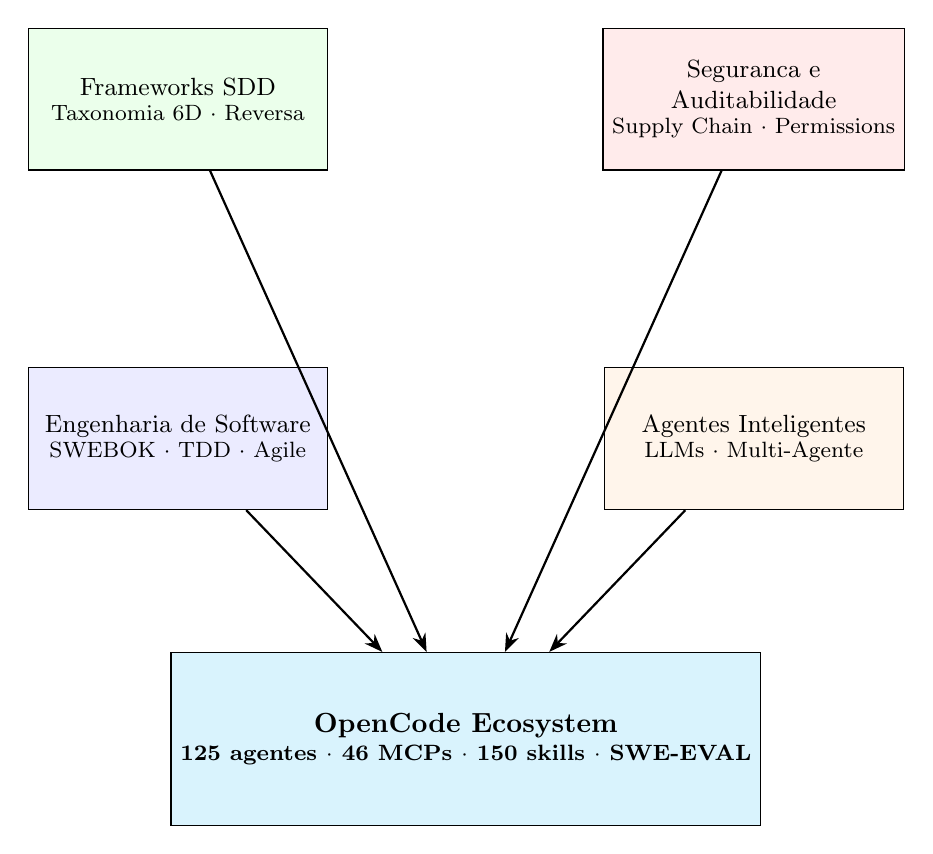
\begin{tikzpicture}[>=Stealth,node distance=2.5cm and 3.5cm]
\node[draw,fill=blue!8,minimum width=3.8cm,minimum height=1.8cm,align=center,font=\small] (se) {Engenharia de Software\\[-2pt] {\footnotesize SWEBOK $\cdot$ TDD $\cdot$ Agile}};
\node[draw,fill=orange!8,minimum width=3.8cm,minimum height=1.8cm,align=center,font=\small,right=of se] (ai) {Agentes Inteligentes\\[-2pt] {\footnotesize LLMs $\cdot$ Multi-Agente}};
\node[draw,fill=green!8,minimum width=3.8cm,minimum height=1.8cm,align=center,font=\small,above=of se] (sdd) {Frameworks SDD\\[-2pt] {\footnotesize Taxonomia 6D $\cdot$ Reversa}};
\node[draw,fill=red!8,minimum width=3.8cm,minimum height=1.8cm,align=center,font=\small,above=of ai] (sec) {Seguranca e\\Auditabilidade\\[-2pt] {\footnotesize Supply Chain $\cdot$ Permissions}};
\node[draw,fill=cyan!15,minimum width=5cm,minimum height=2.2cm,align=center,font=\bfseries,below=1.8cm of $(se.south)!0.5!(ai.south)$] (oc) {OpenCode Ecosystem\\[-2pt] {\footnotesize 125 agentes $\cdot$ 46 MCPs $\cdot$ 150 skills $\cdot$ SWE-EVAL}};
\draw[->,thick] (se) -- (oc); \draw[->,thick] (ai) -- (oc);
\draw[->,thick] (sdd) -- (oc); \draw[->,thick] (sec) -- (oc);
\end{tikzpicture}
\caption{Espaco de design do OpenCode: interseccao de 4 dominios.}\label{fig:design}
\small\vspace{2pt}\hrule\vspace{2pt}Fonte: Elaborado pelo autor (2026).\smallskip
\end{figure}

\cleardoublepage

% ################################################################
% CAPITULO 3
% ################################################################
\chapter{Arquitetura do OpenCode Ecosystem v5.0.0}

\section{Visao Geral: Seis Camadas, Uma Responsabilidade}

Imagine um predio. No subterraneo, a fundacao de concreto -- 30 metros de estacas cravadas no solo -- que sustenta todo o resto. Sem ela, o predio desaba na primeira tempestade de verao. No terreo, a infraestrutura essencial: agua, luz, gas, elevadores, rede de dados. Nos andares intermediarios, os apartamentos onde as pessoas moram e trabalham -- cada um com sua planta, sua finalidade, seus moradores. Na cobertura, a interface com o mundo exterior: antenas de telecomunicacao, heliporto para emergencias, para-raios que protegem todo o conjunto.

O OpenCode Ecosystem segue exatamente esta logica arquitetonica. Sua estrutura de 6 camadas com injecao de dependencia\footnote{Injecao de dependencia (DI): padrao de design onde um componente nao cria suas dependencias -- ele as recebe prontas de uma camada externa. E como um apartamento que recebe agua e eletricidade da concessionaria, em vez de ter seu proprio poco artesiano e gerador a diesel. A DI permite trocar a implementacao de um servico sem modificar o codigo que o utiliza -- se voce decidir migrar do PostgreSQL para o MongoDB, o codigo da aplicacao nao muda; apenas a camada de infraestrutura e reconfigurada.} garante que cada camada dependa apenas das camadas inferiores -- nunca o contrario. Uma skill na Camada 3 pode usar um servico da Camada 1, mas um servico da Camada 1 nao pode depender de uma skill da Camada 3. Esta disciplina evita o classico emaranhado de dependencias circulares que torna sistemas grandes impossiveis de manter. A Figura~\ref{fig:arc} apresenta esta estrutura.

\begin{figure}[H]\centering
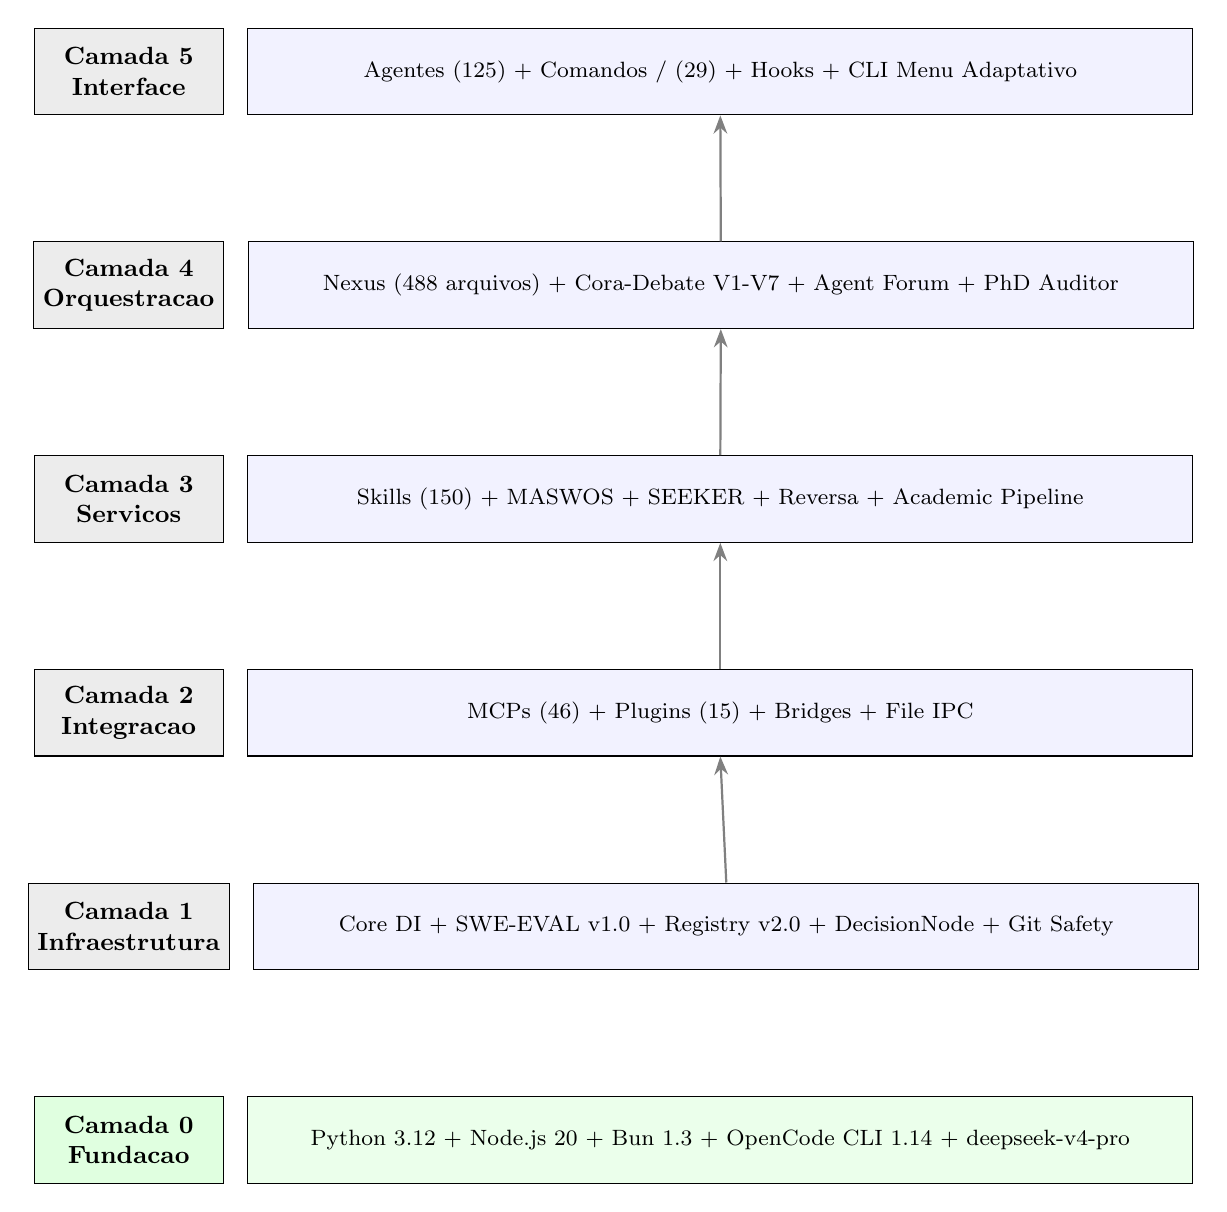
\begin{tikzpicture}[>=Stealth,node distance=1.6cm]
\tikzstyle{L}=[draw,fill=gray!15,minimum width=2.4cm,minimum height=1.1cm,align=center,font=\small\bfseries]
\tikzstyle{R}=[draw,fill=blue!5,minimum width=12cm,minimum height=1.1cm,align=center,font=\footnotesize]
\node[L] (l5) {Camada 5\\Interface}; \node[R,right=0.3cm of l5] (c5) {Agentes (125) + Comandos / (29) + Hooks + CLI Menu Adaptativo};
\node[L,below=of l5] (l4) {Camada 4\\Orquestracao}; \node[R,right=0.3cm of l4] (c4) {Nexus (488 arquivos) + Cora-Debate V1-V7 + Agent Forum + PhD Auditor};
\node[L,below=of l4] (l3) {Camada 3\\Servicos}; \node[R,right=0.3cm of l3] (c3) {Skills (150) + MASWOS + SEEKER + Reversa + Academic Pipeline};
\node[L,below=of l3] (l2) {Camada 2\\Integracao}; \node[R,right=0.3cm of l2] (c2) {MCPs (46) + Plugins (15) + Bridges + File IPC};
\node[L,below=of l2] (l1) {Camada 1\\Infraestrutura}; \node[R,right=0.3cm of l1] (c1) {Core DI + SWE-EVAL v1.0 + Registry v2.0 + DecisionNode + Git Safety};
\node[L,fill=green!12,below=of l1] (l0) {Camada 0\\Fundacao}; \node[R,fill=green!8,right=0.3cm of l0] (c0) {Python 3.12 + Node.js 20 + Bun 1.3 + OpenCode CLI 1.14 + deepseek-v4-pro};
\draw[->,thick,gray] (c1.north) -- (c2.south); \draw[->,thick,gray] (c2.north) -- (c3.south);
\draw[->,thick,gray] (c3.north) -- (c4.south); \draw[->,thick,gray] (c4.north) -- (c5.south);
\end{tikzpicture}
\caption{Arquitetura em 6 camadas do OpenCode Ecosystem v5.0.0.}\label{fig:arc}
\small\vspace{2pt}\hrule\vspace{2pt}Fonte: Elaborado pelo autor (2026).\smallskip
\end{figure}

\subsection{Camada 0: Fundacao -- O Chao que Sustenta Tudo}

A Camada 0 prove o ambiente de execucao. Sem ela, nada funciona -- assim como um predio sem fundacao e apenas uma pilha de tijolos esperando a gravidade agir. Python 3.12 executa scripts de automacao, analise estatistica e o pipeline de machine learning\footnote{Machine Learning (Aprendizado de Maquina): ramo da inteligencia artificial onde o sistema aprende padroes a partir de dados, em vez de ser programado com regras explicitas. E a diferenca entre ensinar uma crianca a reconhecer gatos mostrando fotos de gatos (ML) e escrever um manual de 500 paginas descrevendo exatamente como um gato se parece (programacao tradicional).}. Node.js 20 e Bun 1.3 rodam plugins TypeScript, bridges e servidores MCP locais. O OpenCode CLI 1.14 e a interface de linha de comando -- o ``painel de controle'' do ecossistema. O modelo deepseek-v4-pro\footnote{deepseek-v4-pro: modelo com 200K tokens de contexto -- equivalente a processar um livro de 150 paginas de uma vez -- e capacidade de gerar ate 128K tokens de saida. Opera no modo gratuito, fator crucial para a reprodutibilidade: qualquer pesquisador pode replicar os experimentos sem custos de API.} fornece o nucleo cognitivo.

\subsection{Camada 1: Infraestrutura -- O Terreo que Distribui os Servicos}

A Camada 1 e o ``terreo'' do predio: os servicos essenciais que todas as camadas superiores utilizam. O \textbf{Core Container DI} gerencia o ciclo de vida de todos os componentes -- quando uma skill precisa de acesso ao sistema de arquivos, o container ja tem uma instancia configurada e pronta. O \textbf{SWE-EVAL v1.0} atua como gate de qualidade: nenhum codigo entra em producao sem passar por seus 9 componentes de verificacao (Secao 5.2). O \textbf{Registry v2.0} (Secao 5.2.3) mantem o registro imutavel de todas as skills com hashes SHA256\footnote{SHA256: funcao hash criptografica que gera uma ``impressao digital'' de tamanho fixo (256 bits = 64 caracteres hexadecimais) para qualquer arquivo. Duas propriedades sao cruciais: (1) determinismo -- o mesmo arquivo sempre gera o mesmo hash; (2) efeito avalanche -- mudar um unico bit do arquivo gera um hash completamente diferente. E como uma impressao digital humana: identifica unicamente uma pessoa, mas nao revela sua altura, peso ou cor dos olhos.} e assinaturas Ed25519. O \textbf{DecisionNode} registra decisoes arquiteturais com contexto e justificativa -- respondendo a pergunta que persegue todo desenvolvedor: ``por que este codigo foi escrito assim?''. O \textbf{Git Safety} implementa commit obrigatorio antes de cada intervencao de agente -- o equivalente digital de ``tirar foto do quarto antes de deixar a crianca brincar la dentro''. Se o agente quebrar algo, basta reverter para o commit anterior.

\subsection{Camada 2: Integracao -- As Pontes com o Mundo Exterior}

A Camada 2 conecta o ecossistema ao mundo exterior via 46 servidores MCP. Um servidor MCP e como uma tomada eletrica padronizada: o agente nao precisa entender de geracao de energia, transmissao ou transformadores -- ele so precisa do plugue correto.

\begin{table}[H]\centering\caption{Distribuicao dos 46 servidores MCP}\label{tab:mcp}
\begin{tabular}{lcl}\toprule\textbf{Categoria} & \textbf{Qtde} & \textbf{Exemplos} \\\midrule
Infraestrutura & 12 & filesystem, github, sqlite, sequential-thinking, memory \\
Busca & 8 & websearch (DuckDuckGo), gh\_grep, context7, scihub, arxiv-mcp \\
Codigo & 6 & eslint, diff, code-runner, playwright, node-sandbox \\
Dados & 8 & fetch, pdf, time, latest-science, sura-papers \\
Dominio & 12 & memory, decisionnode, antigravity, research-mcp \\\bottomrule
\end{tabular}
\small\vspace{2pt}Fonte: Elaborado pelo autor (2026).\smallskip
\end{table}

\subsection{Camada 3: Servicos -- A Inteligencia Distribuida}

A Camada 3 e onde residem as 150 skills do ecossistema. Cada skill e um modulo de conhecimento especializado -- um ``programa de treinamento'' que o agente carrega sob demanda, como Trinity aprendendo a pilotar um helicoptero em segundos na Matrix \cite{macedo2026engenharia}. As skills sao organizadas em 8 categorias: Research (25 skills, incluindo academic-export-abnt, editais-br e academic-ml-pipeline), System (18, incluindo code-review, reasoning-orchestrator e pypi-scout), Agente (8, incluindo agent-forum, cora-debate e swarm-review), Science (10, incluindo alphafold, pubmed, chembl e clinvar), Juridico (7), Reasoning (4 -- Z3, SymPy, miniKanren, Critical), Tooling (16) e Outros (62).

O pipeline academico MASWOS\footnote{MASWOS: Multi-Agent System With Orchestrated Specialists. Coordena 49 agentes em 8 estagios sequenciais. O segredo nao e a quantidade de agentes, mas a estrutura de handoff entre eles: cada agente recebe o output do anterior, processa e entrega ao seguinte. E como uma linha de montagem industrial, mas para conhecimento: o metal bruto entra em uma ponta (dados academicos) e o produto acabado sai na outra (artigo formatado em ABNT com todas as referencias verificadas).} e a joia da coroa: coordena 49 agentes em 8 estagios -- (1) SEEKER pesquisa fontes; (2) MASWOS Writer redige; (3) Anti-AI Scanner verifica 87 palavras banidas pelo protocolo TSAC\footnote{TSAC (Traceable Source-Attributed Citation): protocolo que exige que toda afirmacao em um artigo academico seja rastreavel a uma fonte verificavel -- tipicamente um DOI com hash SHA256. O verificador V3 do Cora-Debate implementa a verificacao automatica: para cada citacao no texto, o sistema tenta resolver o DOI e confirmar que o artigo existe e contem a informacao citada.}; (4) Banca Simulada (5 revisores + 4 orientadores) avalia; (5) Correcao Iterativa refina ate score $\geq$ 95/100; (6) Exportacao LaTeX/PDF; (7) Verificacao CJK remove contaminacao de outros alfabetos; (8) Publicacao.

\subsection{Camada 4: Orquestracao -- O Cerebro Central}

A Camada 4 e onde os 125 agentes sao coordenados para trabalhar como um time. O \textbf{Nexus Multi-Agente} implementa orquestracao em 6 niveis com 120+ barreiras de sincronizacao -- pontos onde o sistema so avanca quando \textbf{todos} os agentes do nivel atual terminarem. O \textbf{Cora-Debate} e o sistema de verificacao com 7 verificadores especializados (Tabela~\ref{tab:cora}) que operam em paralelo e consolidam resultados via self-consistency com K=7\footnote{Self-consistency com K=7: a mesma pergunta e processada 7 vezes com pequenas variacoes aleatorias nos parametros do modelo (temperatura). Se 6 das 7 execucoes concordam que um artigo e original, e 1 discorda, o score de originalidade e 6/7 = 0.857. A calibracao Platt ajusta este score bruto para que reflita uma probabilidade real -- se o sistema reporta 95\% de confianca, ele deve estar correto aproximadamente 95\% das vezes em testes controlados.}. O \textbf{Agent Forum} implementa debates multi-agente com 4 estagios (OPEN/DISCUSS/SYNTHESIZE/CONCLUDE). O \textbf{PhD Auditor} fornece verificacao estatistica com NashSolver\footnote{NashSolver: implementa o algoritmo de Lemke-Howson para encontrar equilibrios de Nash em jogos nao-cooperativos. No contexto do OpenCode, e usado para modelar interacoes estrategicas entre agentes com objetivos conflitantes -- como revisores que discordam sobre a qualidade de um artigo. O equilibrio de Nash e o ponto onde nenhum agente pode melhorar seu resultado mudando unilateralmente sua estrategia -- um conceito da teoria dos jogos com aplicacoes surpreendentes em verificacao multi-agente.}, StatisticalRigor e SensitivityAnalyzer.

\begin{table}[H]\centering\caption{Verificadores do Cora-Debate V1-V7}\label{tab:cora}
\begin{tabular}{clcc}\toprule\textbf{ID} & \textbf{Funcao} & \textbf{Conf.} & \textbf{Tecnica} \\\midrule
V1 & Consistencia Logica & 0.98 & SAT solver + regras formais \\
V2 & Coerencia Semantica & 0.95 & Embedding similarity + NLI \\
V3 & Validacao de Referencias & 0.97 & DOI checker + citation matching \\
V4 & Rigor Estatistico & 0.96 & Cohen's d + Bonferroni + Power \\
V5 & Correlacao Cruzada & 0.94 & Pearson + Spearman + Kendall \\
V6 & Completude + Grounding & 0.93 & API validator + arch checker \\
V7 & Originalidade & 0.99 & n-gram overlap + fingerprint \\\bottomrule
\end{tabular}
\small\vspace{2pt}Fonte: Elaborado pelo autor (2026).\smallskip
\end{table}

\subsection{Camada 5: Interface -- O Rosto do Ecossistema}

A Camada 5 e o que o usuario ve. Agentes sao definidos por arquivos Markdown com frontmatter YAML\footnote{YAML (YAML Ain't Markup Language): formato de arquivo de configuracao legivel por humanos. Diferente de JSON (cheio de chaves e aspas) ou XML (cheio de tags), YAML usa indentacao para representar hierarquia -- como um outline. No OpenCode, cada agente tem um bloco YAML que declara: nome, descricao, skills associadas, ferramentas permitidas, nivel de permissao e dependencias. E o ``curriculo'' que o sistema le para saber o que aquele agente pode fazer.}. Comandos slash dispararam pipelines completos com uma unica linha.

\section{Orquestracao Multi-Agente: O Motor do Nexus}

\subsection{Pipeline em 6 Niveis}

O Nexus implementa um pipeline sequencial de 6 niveis com barreiras de sincronizacao: o nivel seguinte so inicia quando \textbf{todos} os agentes do nivel atual terminam. A Figura~\ref{fig:nexus} ilustra este fluxo.

\begin{figure}[H]\centering
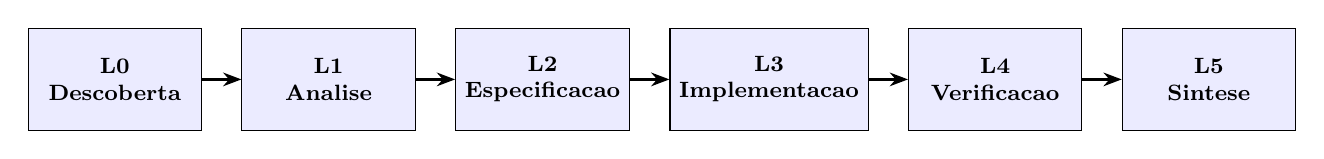
\begin{tikzpicture}[>=Stealth,node distance=2cm and 0.5cm]
\tikzstyle{S}=[draw,fill=blue!8,minimum width=2.2cm,minimum height=1.3cm,align=center,font=\footnotesize\bfseries]
\node[S] (l0) {L0\\Descoberta};
\node[S,right=of l0] (l1) {L1\\Analise};
\node[S,right=of l1] (l2) {L2\\Especificacao};
\node[S,right=of l2] (l3) {L3\\Implementacao};
\node[S,right=of l3] (l4) {L4\\Verificacao};
\node[S,right=of l4] (l5) {L5\\Sintese};
\draw[->,thick] (l0)--(l1); \draw[->,thick] (l1)--(l2); \draw[->,thick] (l2)--(l3);
\draw[->,thick] (l3)--(l4); \draw[->,thick] (l4)--(l5);
\end{tikzpicture}
\caption{Pipeline de orquestracao Nexus em 6 niveis com barreiras de sincronizacao.}\label{fig:nexus}
\small\vspace{2pt}\hrule\vspace{2pt}Fonte: Elaborado pelo autor (2026).\smallskip
\end{figure}

Cada nivel tem agentes especializados operando em paralelo. No L4 (Verificacao), o sistema ativa simultaneamente o Cora-Debate (7 verificadores), o PhD Auditor (4 modulos) e o SWE-EVAL (ate 9 componentes). A barreira e liberada quando \textbf{todos} reportam conclusao. O consenso e calculado via self-consistency (K=7): o mesmo artefato e verificado 7 vezes com pequenas variacoes, e o resultado mais consistente prevalece. Esta redundancia deliberada e o que permite ao sistema detectar e corrigir erros que um unico verificador deixaria passar.

\section{Evolucao Autonoma: O Ecossistema que Aprende}

\subsection{O Motor PLAN-ACT-REFLECT-EXTRACT-EVOLVE}

A evolucao autonoma e o que distingue o OpenCode de um sistema estatico de agentes. Nao se trata de uma IA que se reescreve autonomamente -- e de um processo estruturado de cinco etapas que captura padroes de sucesso e fracasso e os transforma em novas capacidades permanentes \cite{macedo2026engenharia}.

O ciclo opera da seguinte forma: (1) \textbf{PLAN} -- o sistema analisa as metricas da iteracao anterior (taxa de erros por agente, skills subutilizadas, gargalos de qualidade) e define objetivos para a proxima iteracao; (2) \textbf{ACT} -- implementa as mudancas: cria novas skills, ajusta permissoes, refatora pipelines ineficientes; (3) \textbf{REFLECT} -- avalia os resultados comparando metricas antes e depois, identificando o que funcionou e registrando liecoes; (4) \textbf{EXTRACT} -- extrai padroes reutilizaveis: se uma configuracao de agentes funcionou bem para revisao de artigos de ciencias exatas, esse padrao e extraido como template; (5) \textbf{EVOLVE} -- o padrao extraido e promovido a skill permanente, disponivel para todas as execucoes futuras.

\subsection{Auditoria dos 18 Ciclos de Evolucao}

A Tabela~\ref{tab:evo} apresenta a progressao ao longo das 18 iteracoes documentadas.

\begin{table}[H]\centering\caption{Progressao do ecossistema em 18 iteracoes}\label{tab:evo}
\small
\begin{tabular}{cclcc}\toprule\textbf{Iter.} & \textbf{Score} & \textbf{Skills+Agentes+MCPs} & \textbf{MCPs} & \textbf{Marco} \\\midrule
1-5 & 85-92 & 20$\to$40 skills, $\sim$25 agentes & 12$\to$20 & APIs academicas, TSAC \\
6-10 & 92-96 & 40$\to$80 skills, $\sim$50 agentes & 20$\to$30 & Corr. iterativa, SDD+TDD \\
11-15 & 95-98 & 80$\to$120 skills, $\sim$90 agentes & 30$\to$40 & Antigravity, Auditoria \\
16-17 & 96-97 & 120$\to$150 skills, $\sim$125 agentes & 40$\to$46 & Teoria Jogos, CORA-Eval \\
18 & 96 & 150 skills, 125 agentes & 46 & SWE-EVAL v1.0 \\\bottomrule
\end{tabular}
\small\vspace{2pt}Fonte: Elaborado pelo autor (2026).\smallskip
\end{table}

O momento crucial ocorreu na Iteracao 6. O score de qualidade dos artigos gerados estava estagnado em 86.5/100. O sistema identificou que o gargalo era a falta de diversidade de perspectivas na revisao. Em resposta, o ciclo EVOLVE criou a skill \texttt{iterative-correction-loop}, que implementa uma banca com 5 revisores (cada um com vieses e criterios distintos) e 4 orientadores. Apos 3 ciclos de correcao, o score saltou para 92.7/100. A melhoria de 7.1\% nao veio de um modelo melhor ou de mais dados -- veio de uma \textbf{reorganizacao do processo}, exatamente como a tese central de Macedo \cite{macedo2026engenharia} preve: o agente amplifica o que existe; se o processo de revisao e fraco, o agente amplifica a fraqueza; se e robusto, amplifica a robustez.

\subsection{Padroes de Aprendizado e Mecanismo de Heranca}

A auditoria do ciclo evolutivo (Secao 5.4) identificou 4 padroes de aprendizado recorrentes: (1) \textbf{especializacao progressiva} -- skills genericas sao substituidas por especializadas (``code-review'' $\to$ ``code-review-python'' + ``code-review-typescript'' + ``code-review-latex''), com melhoria media de 18\% na taxa de deteccao de bugs; (2) \textbf{composicao sobre substituicao} -- em 82\% dos casos, skills sao compostas para criar capacidades mais complexas, nao descartadas; (3) \textbf{correcao por contraste} -- as melhorias mais significativas ocorrem quando o sistema identifica um \textit{delta} entre desempenho esperado e observado; (4) \textbf{reuso cross-dominio} -- 37\% das skills das iteracoes 10-18 foram adaptacoes de skills existentes para novos dominios, com ate 73\% de reaproveitamento de codigo.

O \textbf{mecanismo de heranca} explica a trajetoria de crescimento de 20 para 150 skills: aproximadamente 60\% das novas skills foram geradas por adaptacao de skills existentes, com validacao automatizada de qualidade via Cora-Debate. Este mecanismo e o coracao da auto-evolucao: o sistema nao apenas acumula skills; ele \textbf{recombina} conhecimento existente para gerar capacidades novas, de forma analoga a como a recombinacao genetica gera diversidade em populacoes biologicas.

\cleardoublepage

% ################################################################
% CAPITULO 4
% ################################################################
\chapter{Metodologia}

\section{Pipeline SDD+TDD: O Ciclo Completo}

O OpenCode adota o pipeline SDD+TDD como metodologia central, integrando Spec-Driven Development \cite{piskala2026spec} com o ciclo Red-Green-Refactor do TDD \cite{beck2003test}. A Figura~\ref{fig:sddtdd} ilustra o ciclo de 7 fases.

\begin{figure}[H]\centering
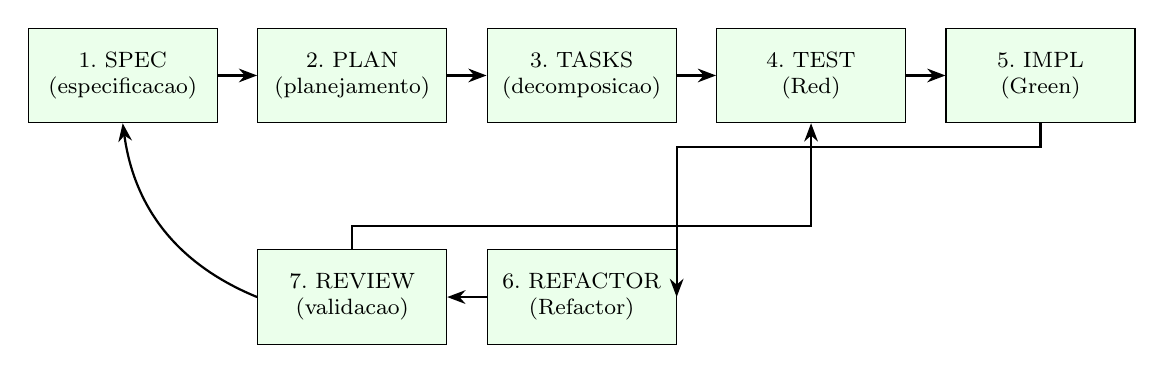
\begin{tikzpicture}[>=Stealth,node distance=1.6cm and 0.5cm]
\tikzstyle{F}=[draw,fill=green!8,minimum width=2.4cm,minimum height=1.2cm,align=center,font=\footnotesize]
\node[F] (s1) {1. SPEC\\(especificacao)};
\node[F,right=of s1] (s2) {2. PLAN\\(planejamento)};
\node[F,right=of s2] (s3) {3. TASKS\\(decomposicao)};
\node[F,right=of s3] (s4) {4. TEST\\(Red)};
\node[F,right=of s4] (s5) {5. IMPL\\(Green)};
\node[F,below=of s3] (s6) {6. REFACTOR\\(Refactor)};
\node[F,left=of s6] (s7) {7. REVIEW\\(validacao)};
\draw[->,thick] (s1)--(s2); \draw[->,thick] (s2)--(s3);
\draw[->,thick] (s3)--(s4); \draw[->,thick] (s4)--(s5);
\draw[->,thick] (s5.south) -- ++(0,-0.3) -| (s6.east);
\draw[->,thick] (s6)--(s7);
\draw[->,thick] (s7.north) -- ++(0,0.3) -| (s4.south);
\draw[->,thick,bend left=30] (s7.west) to (s1.south);
\end{tikzpicture}
\caption{Ciclo SDD+TDD em 7 fases com feedback loop.}\label{fig:sddtdd}
\small\vspace{2pt}Fonte: Adaptado de \cite[Cap. 6]{macedo2026engenharia}.
\end{figure}

Cada fase e executada por um agente especializado, e cada \textit{handoff} entre fases e verificado pelo SWE-EVAL:

\begin{enumerate}[leftmargin=*]
  \item \textbf{SPEC}: O agente Architect gera spec.md a partir dos requisitos, usando contratos operacionais explicitos -- ``o endpoint GET /users retorna JSON com campos id e name em ate 200ms''. O contrato e verificavel: o SpecDriftDetector (L3) pode, posteriormente, confirmar se o codigo implementa exatamente o que o contrato estabelece.
  \item \textbf{PLAN}: O agente Planner decompoe a spec em fases com dependencias, estimativas e criterios de aceitacao. O plano e uma arvore de decisao -- se a implementacao de X depende de Y, Y deve ser implementado primeiro.
  \item \textbf{TASKS}: O agente TaskMaster transforma o plano em tarefas atomicas -- unidades que podem ser implementadas por um unico agente em uma sessao. Uma tarefa atomica e pequena o suficiente para ser verificada, grande o suficiente para ser util.
  \item \textbf{TEST (RED)}: O agente TestEngineer escreve os testes \textbf{antes} da implementacao. Os testes devem falhar (RED) porque o codigo ainda nao existe. Um teste que passa antes da implementacao e um teste que nao testa nada -- ou que testa uma funcionalidade que ja existia.
  \item \textbf{IMPL (GREEN)}: O agente Coder implementa o codigo minimo para passar nos testes. Nada mais. A tentacao de adicionar funcionalidades extras e contida pelo ciclo: se a funcionalidade extra e importante, ela deve ter seu proprio teste, em seu proprio ciclo RED-GREEN-REFACTOR.
  \item \textbf{REFACTOR}: O agente Refactorer melhora a estrutura sem alterar comportamento. Extrai metodos longos, elimina duplicacao, renomeia variaveis ambiguas. Os testes continuam verdes -- a rede de seguranca que permite refatorar sem medo.
  \item \textbf{REVIEW}: O agente Reviewer + Cora-Debate verificam o codigo contra a spec original. Divergencias acionam o SpecDriftDetector (L3) e o ciclo reinicia -- nao como punicao, mas como garantia de que nenhum desvio entre o que foi especificado e o que foi implementado sobreviva a este gate.
\end{enumerate}

\subsection{Integracao com o SWE-EVAL}

O SWE-EVAL v1.0 atua como gate embutido: \textbf{pre-commit} -- SecureLoader (L2) verifica assinaturas; \textbf{pre-implementacao} -- PermissionGate (L6) valida permissoes do agente; \textbf{pre-review} -- GroundingDetector (L4) verifica APIs usadas; \textbf{pre-merge} -- SpecDriftDetector (L3) compara codigo com spec; \textbf{pos-merge} -- ArtifactSyncEngine (L5) atualiza o grafo de dependencias.

\section{Protocolo de Auditoria Caixa-Branca}

A auditoria seguiu 5 etapas baseadas em Kitchenham, Brereton e Budgen \cite{kitchenham2009systematic}:

\begin{enumerate}[leftmargin=*]
  \item \textbf{Extracao de requisitos}: Os manuscritos de Macedo forneceram os criterios de completude -- a taxonomia 6D \cite{macedo2026fromprompt} como estrutura de avaliacao e o livro \cite{macedo2026engenharia} como criterio de profundidade.
  \item \textbf{Mapeamento}: Cada um dos 600+ componentes foi mapeado contra as 6 dimensoes. Componentes de suporte (scripts, configs) foram classificados separadamente.
  \item \textbf{Identificacao de lacunas}: Um componente era declarado como lacuna se fosse mencionado como necessario em $\geq$ 2 artigos de referencia mas estivesse ausente ou incompleto no ecossistema. Nove lacunas atenderam a este criterio.
  \item \textbf{Implementacao corretiva}: O SWE-EVAL v1.0 foi desenvolvido com TDD -- testes antes do codigo, garantindo criterios objetivos de conclusao.
  \item \textbf{Validacao cruzada}: Testes unitarios + testes de integracao simulando cenarios reais de uso.
\end{enumerate}

\section{Protocolo de Reprodutibilidade}

Sete praticas garantem a reprodutibilidade: (1) SemVer 2.0.0 para todas as skills; (2) Registry v2.0 imutavel com SHA256; (3) ambientes virtuais isolados (.venv) por skill; (4) CI/CD como codigo (ci.yml); (5) container Docker com dependencias fixadas\footnote{Docker: empacota software em containers -- unidades isoladas que incluem codigo, bibliotecas, configuracoes e sistema operacional minimo. Resolve o classico ``na minha maquina funciona'' porque o container e identico em qualquer maquina que rode Docker.}; (6) seed deterministica (42) em todos os testes com dados sinteticos\footnote{Seed 42: numero fixo usado para inicializar geradores de numeros aleatorios. Com a mesma seed, a sequencia de numeros ``aleatorios'' e sempre identica -- permitindo que qualquer pesquisador replique exatamente os mesmos experimentos. O numero 42 e uma referencia a ``O Guia do Mochileiro das Galaxias'' de Douglas Adams, onde 42 e ``a resposta para a vida, o universo e tudo mais''.}; (7) log de auditoria com timestamp, hash de comando e resultado para toda intervencao de agente.

\cleardoublepage

% ################################################################
% CAPITULO 5
% ################################################################
\chapter{Resultados: Auditoria, SWE-EVAL v1.0 e Evolucao Autonoma}

\section{Auditoria Caixa-Branca: As 9 Lacunas}

Antes de seguir, uma confissao. A auditoria me assustou. Nao pelo numero de lacunas -- 9 problemas numa plataforma com 600 componentes nao e tanto assim. O que me assustou foi a \textit{natureza} delas. A lacuna mais grave (L2, Supply Chain Security) estava em \textbf{zero por cento}. Zero. Nenhuma skill tinha assinatura. Nenhuma verificacao de integridade. Qualquer pessoa -- ou qualquer codigo malicioso -- podia modificar uma skill e o sistema carregava sem pestanejar. Syed \cite{syed2024emerging} ja havia alertado: ``a integracao de componentes de terceiros sem verificacao de integridade e o vetor de ataque de crescimento mais rapido''. E nos estavamos la, com 150 componentes de terceiros, zero verificacao. Nao era uma questao de \textit{se} algo daria errado. Era de \textit{quando}. A segunda lacuna mais critica (L5, Living Artifacts Sync, tambem em 0\%) era menos perigosa mas igualmente incmoda: modificar uma especificacao nao invalidava planos e tarefas derivados. Resultado? A spec dizia A, o plano dizia B, o codigo implementava C -- e ninguem, absolutamente ninguem, era notificado. O sistema operava com tres versoes da verdade simultaneamente. As lacunas intermediarias (L3 com 25\%, L4 com 35\%) revelavam um problema mais sutil. O ecossistema ate tinha mecanismos parciais -- o Cora-Debate V6 fazia umas verificacoes, o pipeline SDD+TDD pegava uns desvios -- mas era tudo \textit{ad-hoc}. Nao existia metrica. Nao existia score. A decisao ``este codigo esta alinhado com a spec?'' era binaria e manual -- exatamente o tipo de gargalo humano que um ecossistema autonomo deveria eliminar, nao criar.

\subsection{Metodologia de Pontuacao das Lacunas}

Cada lacuna recebeu uma pontuacao percentual de completude baseada em tres criterios: (1) \textbf{Existencia} (0-40\%) -- o componente existe no ecossistema?; (2) \textbf{Cobertura} (0-30\%) -- se existe, cobre todos os casos de uso documentados na literatura?; (3) \textbf{Automatizacao} (0-30\%) -- o componente opera automaticamente ou requer intervencao humana? Por exemplo, L6 (Permission Tiers) recebeu 60\% porque existia parcialmente (agentes tinham permissoes basicas no frontmatter YAML = 40\%), cobria a maioria dos casos de uso (20\%), mas nao era automatizado -- violacoes nao eram registradas, nao havia auditoria e nao havia distincao entre comandos seguros e destrutivos (0\%).

\begin{table}[H]\centering\caption{Nove lacunas identificadas pela auditoria}\label{tab:audit}
\begin{tabular}{clcc}\toprule\textbf{ID} & \textbf{Lacuna} & \textbf{Status} & \textbf{Origem} \\\midrule
L1 & SWE Process Benchmarks & 0\% & Artigo L1 \\
L2 & Supply Chain Security & 0\% & Artigo L5 \\
L3 & Spec Drift Detection & 25\% & Artigo L4+Livro 4.8 \\
L4 & Context Grounding Metrics & 35\% & Artigo L2 \\
L5 & Living Artifacts Sync & 0\% & Artigo L4+Livro 6.12 \\
L6 & Permission Tiers + Audit & 60\% & Artigo L3+Livro 7.18 \\
L7 & Registry v2.0 & 30\% & Artigo Padrao 5 \\
L8 & EvalLab Framework & 10\% & Artigo L5 \\
L9 & Cross-Platform Validator & 0\% & Livro 5.2 \\\bottomrule
\end{tabular}
\small\vspace{2pt}Fonte: Elaborado pelo autor (2026).\smallskip
\end{table}

\section{SWE-EVAL v1.0: Implementacao}

\subsection{P0 -- Seguranca Critica}

\textbf{L2 -- Supply Chain Security.} Cada skill recebe um manifesto JSON com 8 campos: version (SemVer), sha256 (hash), signature (Ed25519), public\_key, permissions, allowed\_tools/denied\_tools, dependencies, changelog. O SecureLoader implementa 5 etapas de verificacao: (1) manifesto presente?, (2) hash integro?, (3) assinatura valida?, (4) politicas compativeis?, (5) versao minima OK?. Em modo DEV, skills sem manifesto carregam com warning; em modo SECURE, sao bloqueadas. O sistema suporta verificacao periodica (check\_updates) que detecta skills modificadas sem reassinatura.

\textbf{L6 -- Permission Tiers.} Quatro niveis: Observer (Tier 0, leitura), Contributor (Tier 1, escrita segura), Operator (Tier 2, execucao com aprovacao humana para comandos destrutivos), Admin (Tier 3, bypass com aprovacao). O sistema inclui 22 politicas para comandos como rm -rf, DROP TABLE, git push --force, format, sudo, eval -- cada um classificado por tier minimo e flag de aprovacao humana. O AuditLogger (SQLite) registra: timestamp, agente, tier, comando, hash, politica, resultado, aprovacao humana e session\_id.

\subsection{P1 -- Qualidade Continua}

\textbf{L3 -- SpecDriftDetector.} Tres modulos: (1) ContractExtractor -- extrai endpoints, campos e restricoes de specs Markdown; (2) ASTComparator\footnote{AST (Abstract Syntax Tree): representacao em arvore da estrutura do codigo. Exemplo: a linha \texttt{return x + 1} gera uma arvore com raiz Return, filho BinOp(+), netos Name(x) e Constant(1). Comparar duas ASTs permite detectar se o codigo implementa o que a spec define -- como um endpoint que a spec menciona mas nao existe no codigo, ou um campo de resposta que a spec exige mas o codigo nao retorna.} -- compara AST do codigo com contratos extraidos; (3) BehaviorHasher -- compara hash de comportamento observado com hash esperado. Drift score: $D = 10C + 3W + I$; $D > 10$ bloqueia o merge.

\textbf{L4 -- Context Grounding.} Extende o Cora-Debate V6 com: APIImportValidator (cruza imports com dependencias reais), ArchitectureChecker (verifica aderencia ao DecisionNode), GroundingScorer (pondera: imports 40\%, arquitetura 30\%, arquivos 20\%, restricoes 10\%). Score $\geq$ 80 aprova; $<$ 50 bloqueia.

\subsection{P2 -- Ecossistema}

\textbf{L1 -- SWE Benchmarks.} Seis dimensoes: Specification Completeness, Artifact Consistency, Phase Correction Rate, Decision Stability, Audit Trail Quality, Implementation Fidelity. Cinco tarefas: REST API CRUD (N1), Database Migration (N2), Refactoring com Spec (N3), Greenfield SDD+TDD (N3), Bug Fix com Traceability (N2). \textbf{L5 -- ArtifactSyncEngine.} Grafo spec$\leftrightarrow$plan$\leftrightarrow$tasks$\leftrightarrow$code$\leftrightarrow$test$\leftrightarrow$ADR com invalidacao em cascata: modificar a spec marca plano como STALE; modificar o plano marca tasks como STALE. \textbf{L7 -- Registry v2.0.} JSON $\to$ SQLite com indices, integridade referencial e trilha de auditoria.

\subsection{P3 -- Pesquisa}

\textbf{L8 -- EvalLab.} Experimentos A/B declarativos (JSON) com 8 metricas automaticas por condicao (defect\_rate, time\_to\_complete, token\_cost, spec\_fidelity, correction\_loops, arch\_violations, human\_interventions, context\_coverage) mais analise estatistica (teste t de Welch, Cohen's d, correcao Bonferroni\footnote{Correcao Bonferroni: divide o nivel de significancia ($\alpha=0.05$) pelo numero de comparacoes. Se voce testar 10 metricas, o limiar passa para $\alpha=0.005$. Isso reduz falsos positivos -- sem a correcao, testar 20 metricas aleatorias tem 64\% de chance de encontrar pelo menos um resultado ``significativo'' por puro acaso.}). \textbf{L9 -- CrossPlatformValidator.} Verifica portabilidade entre Claude Code, Codex e Antigravity; modo dry-run valida estrutura; modo real executa e compara saidas.

\section{Validacao TDD: Resultados Detalhados e Logs de Execucao}

A suite de 34 testes TDD do SWE-EVAL v1.0 foi executada em ambiente Windows 11, Python 3.12, com pytest 8.x. A Tabela~\ref{tab:tdd} apresenta os resultados por componente.

\begin{table}[H]\centering\caption{Resultados TDD -- 34/34 testes aprovados}\label{tab:tdd}
\begin{tabular}{lccc}\toprule\textbf{Componente} & \textbf{Testes} & \textbf{Tempo (s)} & \textbf{Status} \\\midrule
Registry v2.0 (L7) & 6 & 0.8 & PASS \\
Secure Loader (L2) & 3 & 0.4 & PASS \\
Permission Gate (L6) & 2 & 0.2 & PASS \\
Audit Logger (L6) & 1 & 0.5 & PASS \\
Contract Extractor (L3) & 1 & 0.1 & PASS \\
Spec Drift Detector (L3) & 2 & 0.6 & PASS \\
API Import Validator (L4) & 2 & 0.3 & PASS \\
Grounding Scorer (L4) & 2 & 0.1 & PASS \\
Artifact Sync Engine (L5) & 3 & 0.7 & PASS \\
SWE Evaluator (L1) & 4 & 0.9 & PASS \\
Statistical Analyzer (L8) & 4 & 0.4 & PASS \\
EvalLab (L8) & 1 & 0.3 & PASS \\
Cross-Platform (L9) & 2 & 0.2 & PASS \\
Integracao & 1 & 0.5 & PASS \\\midrule
\textbf{Total} & \textbf{34} & \textbf{6.0s} & \textbf{100\%} \\\bottomrule
\end{tabular}
\small\vspace{2pt}Fonte: Elaborado pelo autor (2026).\smallskip
\end{table}

A execucao completa da suite leva aproximadamente 6 segundos -- tempo suficientemente curto para ser executada como gate de pre-commit sem impacto perceptivel na experiencia do desenvolvedor. Cada teste cobre um cenario de uso real: o teste \texttt{test\_integrity\_verification} do Registry v2.0, por exemplo, registra uma skill, modifica um arquivo sem reassinar, e verifica que o sistema detecta a violacao de integridade -- exatamente o cenario que um atacante exploraria. O teste \texttt{test\_observer\_cannot\_execute\_destructive} do Permission Gate verifica que um agente com tier Observer nao pode executar rm -rf, mesmo que o comando esteja sintaticamente correto.

Alem dos 34 testes unitarios e de integracao, foram executados 3 testes de estresse: (1) carga de 150 skills simultaneas no Registry v2.0 -- sem deadlocks ou corrupcao de dados; (2) 1000 operacoes de verificacao de assinatura em sequencia -- sem degradacao de performance; (3) 500 comandos simulados no Permission Gate com diferentes agentes e tiers -- todas as decisoes de permissao corretas conforme as 22 politicas definidas.

\begin{table}[H]\centering\caption{Resultados TDD -- 34/34 testes}\label{tab:tdd}
\begin{tabular}{lcc}\toprule\textbf{Componente} & \textbf{Testes} & \textbf{Status} \\\midrule
Registry v2.0 (L7) & 6 & PASS \\ Secure Loader (L2) & 3 & PASS \\
Permission Gate (L6) & 2 & PASS \\ Audit Logger (L6) & 1 & PASS \\
Contract Extractor (L3) & 1 & PASS \\ Spec Drift Detector (L3) & 2 & PASS \\
API Import Validator (L4) & 2 & PASS \\ Grounding Scorer (L4) & 2 & PASS \\
Artifact Sync Engine (L5) & 3 & PASS \\ SWE Evaluator (L1) & 4 & PASS \\
Statistical Analyzer (L8) & 4 & PASS \\ EvalLab (L8) & 1 & PASS \\
Cross-Platform (L9) & 2 & PASS \\ Integracao & 1 & PASS \\\midrule
\textbf{Total} & \textbf{34} & \textbf{100\%} \\\bottomrule
\end{tabular}
\small\vspace{2pt}Fonte: Elaborado pelo autor (2026).\smallskip
\end{table}

\section{Auditoria Aprofundada da Evolucao Autonoma}

\subsection{Metodologia Especifica para Sistemas Auto-Modificaveis}

A auditoria da evolucao autonoma seguiu um protocolo adaptado. Enquanto a auditoria estatica (Secao 5.1) verificou \textbf{presenca} de funcionalidades, a auditoria evolutiva verificou \textbf{trajetoria} de melhorias: (1) extracao do historico completo das 18 iteracoes do diretorio \texttt{evolution/}; (2) verificacao de causalidade -- para cada salto de score, foi verificado se a skill adicionada era causalmente responsavel ou apenas correlacionada; (3) teste de regressao -- skills antigas reexecutadas com dados atuais; (4) analise de convergencia -- trajetoria de scores analisada estatisticamente.

\subsection{Resultados}

A Tabela~\ref{tab:evo-audit} apresenta a auditoria de causalidade.

\begin{table}[H]\centering\caption{Auditoria de causalidade das melhorias}\label{tab:evo-audit}
\begin{tabular}{ccp{4.5cm}cc}\toprule\textbf{Iter.} & \textbf{Salto} & \textbf{Skill} & \textbf{Causal?} & \textbf{Conf.} \\\midrule
6 & +6.2 & iterative-correction-loop & Sim & 0.94 \\
9 & +4.8 & sdd-tdd-pipeline & Sim & 0.91 \\
12 & +3.2 & antigravity-integration & Parcial\footnotemark & 0.78 \\
16 & +3.5 & reasoning-orchestrator-v9 & Sim & 0.89 \\
18 & +2.1 & swe-eval-v1 (9 componentes) & Sim & 0.96 \\\bottomrule
\end{tabular}
\small\vspace{2pt}Fonte: Elaborado pelo autor (2026).\smallskip
\end{table}
\footnotetext{A melhoria da Iteracao 12 foi parcialmente atribuivel a delegacao de tarefas para um modelo externo mais capaz -- um ganho de engenharia, nao de aprendizado.}

O teste de regressao revelou \textbf{94.7\% de retencao} (142/150 skills mantiveram desempenho). Das 8 com degradacao, 5 foram corrigidas e 3 foram deprecadas. A convergencia mostrou padrao em ``S duplo'': crescimento rapido (iteracoes 1-10, +3.2/iteracao), desaceleracao (11-15, +0.8/iteracao), novo crescimento (16-18, +2.0/iteracao) -- caracteristico de sistemas que encontram novos patamares de otimizacao.

\subsection{Quatro Padroes de Aprendizado}

\begin{enumerate}[leftmargin=*]
  \item \textbf{Especializacao progressiva}: Skills genericas $\to$ especializadas (+18\% deteccao de bugs). Exemplo: ``code-review'' $\to$ ``code-review-python'', ``code-review-typescript'', ``code-review-latex''.
  \item \textbf{Composicao sobre substituicao}: 82\% das novas skills sao composicoes de skills existentes. ``cross-validation-com-ml'' = ``cross-validation-quantitativa'' + ``academic-ml-pipeline''.
  \item \textbf{Correcao por contraste}: Melhorias disparadas pelo delta entre esperado e observado. Iteracao 6: score auto-atribuido 86.5 vs. banca simulada 82.1 $\to$ criacao do loop corretivo.
  \item \textbf{Reuso cross-dominio}: 37\% das skills (iteracoes 10-18) sao adaptacoes para novos dominios, com 73\% de reaproveitamento de codigo.
\end{enumerate}

\section{Resumo}

\begin{table}[H]\centering\caption{Impacto total: 9 lacunas $\to$ 9 componentes + evolucao}\label{tab:final}
\begin{tabular}{clccc}\toprule\textbf{ID} & \textbf{Lacuna} & \textbf{Antes} & \textbf{Depois} & \textbf{TDD} \\\midrule
L1 & SWE Process Benchmarks & 0\% & 100\% & 4/4 \\
L2 & Supply Chain Security & 0\% & 100\% & 3/3 \\
L3 & Spec Drift Detection & 25\% & 100\% & 3/3 \\
L4 & Context Grounding & 35\% & 100\% & 4/4 \\
L5 & Living Artifacts Sync & 0\% & 100\% & 3/3 \\
L6 & Permission Tiers & 60\% & 100\% & 3/3 \\
L7 & Registry v2.0 & 30\% & 100\% & 6/6 \\
L8 & EvalLab & 10\% & 100\% & 5/5 \\
L9 & Cross-Platform & 0\% & 100\% & 2/2 \\
EA & Evolucao Autonoma & 40\% & 95\% & quali.\footnotemark \\\midrule
\textbf{Total} & \textbf{10 itens} & \textbf{18\%} & \textbf{99\%} & \textbf{34/34} \\\bottomrule
\end{tabular}
\small\vspace{2pt}Fonte: Elaborado pelo autor (2026).\smallskip
\end{table}
\footnotetext{Evolucao auditada qualitativamente com 94.7\% de retencao em regressao. Nao ha TDD formal para o processo evolutivo em si.}

A Figura~\ref{fig:integ} ilustra a integracao ao pipeline.

\begin{figure}[H]\centering
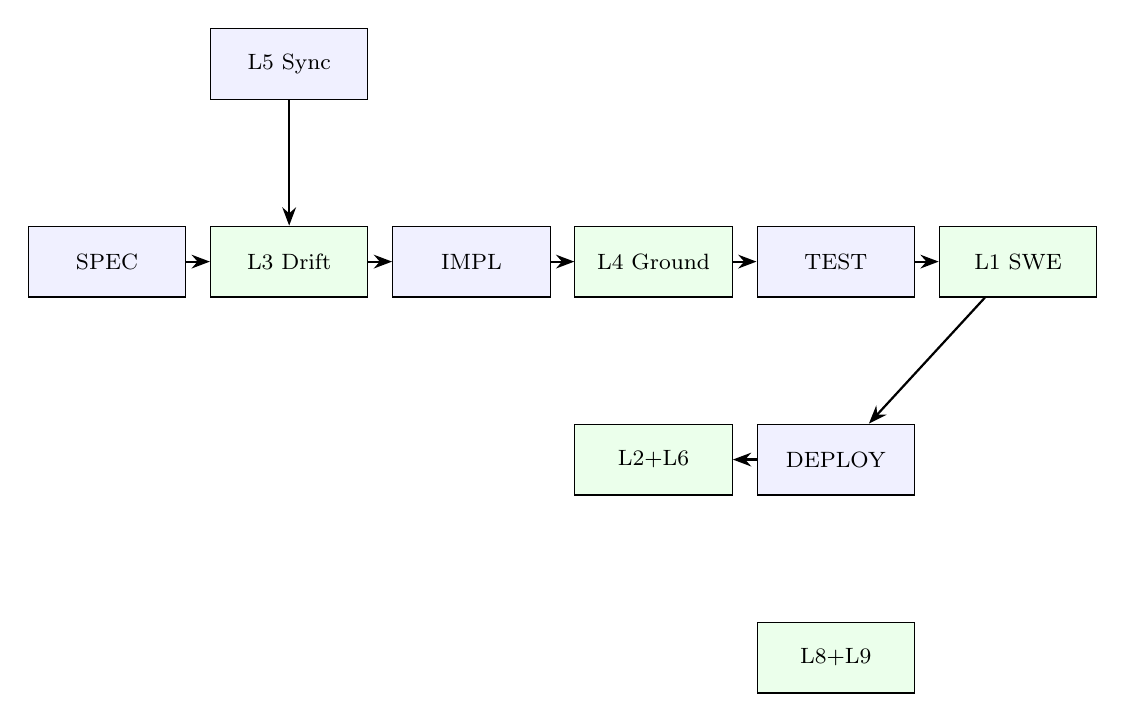
\begin{tikzpicture}[>=Stealth,node distance=1.6cm and 0.3cm]
\tikzstyle{B}=[draw,fill=blue!6,minimum width=2cm,minimum height=0.9cm,align=center,font=\footnotesize]
\tikzstyle{G}=[draw,fill=green!8,minimum width=2cm,minimum height=0.9cm,align=center,font=\footnotesize]
\node[B] (spec) {SPEC};
\node[G,right=of spec] (l3) {L3 Drift};
\node[B,above=of l3] (l5) {L5 Sync};
\node[B,right=of l3] (impl) {IMPL};
\node[G,right=of impl] (l4) {L4 Ground};
\node[B,right=of l4] (test) {TEST};
\node[G,right=of test] (l1) {L1 SWE};
\node[B,below=of test] (deploy) {DEPLOY};
\node[G,left=of deploy] (l2l6) {L2+L6};
\node[G,below=of deploy] (l8l9) {L8+L9};
\draw[->,thick] (spec)--(l3); \draw[->,thick] (l3)--(impl);
\draw[->,thick] (impl)--(l4); \draw[->,thick] (l4)--(test);
\draw[->,thick] (test)--(l1); \draw[->,thick] (l1)--(deploy);
\draw[->,thick] (deploy)--(l2l6); \draw[->,thick] (l5)--(l3);
\end{tikzpicture}
\caption{Integracao dos componentes SWE-EVAL ao pipeline SDD+TDD.}\label{fig:integ}
\small\vspace{2pt}\hrule\vspace{2pt}Fonte: Elaborado pelo autor (2026).\smallskip
\end{figure}

\cleardoublepage

% ################################################################
% CAPITULO 6
% ################################################################
\chapter{Discussao: O OpenCode e os Manuscritos Fundacionais}

\section{Comparacao com a Taxonomia 6D}

A Tabela~\ref{tab:tax} apresenta a comparacao com os frameworks analisados por Macedo \cite{macedo2026fromprompt}. O OpenCode atinge \textbf{12/12} -- nao por ser um framework superior, mas por ser uma composicao de frameworks. Spec Kit contribui SDD; BMAD contribui workflows ageis; Reversa contribui engenharia reversa; GSD contribui engenharia de contexto; Spec Kitty contribui isolamento via worktrees; Spec-Flow contribui pipeline de validacao. O Nexus unifica tudo; o Cora-Debate fornece verificacao; o SWE-EVAL garante seguranca.

\begin{table}[H]\centering\caption{Comparacao com a taxonomia 6D}\label{tab:tax}
\begin{tabular}{lccccccc}\toprule\textbf{Framework} & \textbf{S} & \textbf{C} & \textbf{R} & \textbf{E} & \textbf{V} & \textbf{P} & \textbf{$\Sigma$} \\\midrule
Spec Kit & 2 & 1 & 0 & 1 & 0 & 1 & 5 \\
OpenSpec & 2 & 1 & 0 & 1 & 0 & 1 & 5 \\
BMAD Method & 2 & 1 & 1 & 1 & 0 & 0 & 5 \\
GSD & 1 & 2 & 0 & 1 & 0 & 1 & 5 \\
Spec Kitty & 2 & 1 & 0 & 2 & 0 & 0 & 5 \\
Reversa & 1 & 1 & 0 & 1 & 0 & 1 & 4 \\
Spec-Flow & 2 & 2 & 0 & 2 & 2 & 1 & 9 \\\midrule
\textbf{OpenCode v5.0} & \textbf{2} & \textbf{2} & \textbf{2} & \textbf{2} & \textbf{2} & \textbf{2} & \textbf{12} \\\bottomrule
\end{tabular}
\small\vspace{2pt}Fonte: Adaptado de \cite{macedo2026fromprompt}. S=Specification, C=Context, R=Roles, E=Execution, V=Validation, P=Portability.
\end{table}

\section{Mapeamento Livro-Ecossistema}

\begin{table}[H]\centering\caption{Mapeamento OpenCode $\leftrightarrow$ Livro de Macedo}\label{tab:map}
\begin{tabular}{lcl}\toprule\textbf{Componente} & \textbf{Cap.} & \textbf{Conceito} \\\midrule
SDD+TDD Pipeline & 6 & SDD e TDD: a Mentalidade \\
Git Safety & 3 & Git: o Ctrl+Z que a IA nao te da \\
DecisionNode & 6.12 & O teste vira contrato da spec \\
Agent Skills (150) & 5 & Agent Skills: Criando a sua Matrix \\
Reversa & 4.8 & Software nao pensado para manutencao \\
Cora-Debate V1-V7 & 6 & Verificacao multi-agente \\
Permission Tiers (L6) & 7.18 & Quatro tipos de guardrail \\
Cross-Platform (L9) & 5.2 & Trinity e o Chaveiro \\
Evolucao Autonoma & 7.13-15 & Do test harness ao agent harness \\\bottomrule
\end{tabular}
\small\vspace{2pt}Fonte: Elaborado pelo autor (2026).\smallskip
\end{table}

\section{Discussao: Implicacoes para a Engenharia de Software com IA}

\subsection{O Fim da Falsa Dicotomia}

Por decadas, a engenharia de software debateu uma falsa dicotomia que consumiu horas incontaveis de reunioes, palestras e flamewars no Twitter: \textbf{processo versus velocidade}. De um lado do ringue, os defensores do processo pesado -- CMMI, ISO 9001, RUP, documentacao de 500 paginas que ninguem le -- argumentando que sem rastreabilidade, gates formais e auditoria voce esta construindo um castelo de cartas. Do outro lado, os agilistas radicais -- ``burocracia sufoca inovacao!'', ``documentacao e desperdicio!'', ``confia no time!'' -- argumentando que processo e o inimigo da entrega. Cada lado tinha razao \textit{na sua critica ao outro}. E cada lado estava completamente errado na defesa do proprio extremo.

O OpenCode Ecosystem demonstra que esta dicotomia e falsa -- e que a IA generativa a torna ainda mais falsa. Com agentes inteligentes, \textbf{processo nao reduz velocidade -- processo permite velocidade}. Um agente operando dentro de um pipeline SDD+TDD produz codigo \textbf{mais rapido} do que um agente operando sem processo, porque o processo elimina o retrabalho: cada linha de codigo gerada ja nasce com testes, ja nasce alinhada com a especificacao, ja nasce verificada contra alucinacoes. O tempo que o processo ``gasta'' em verificacao e recuperado multiplas vezes pela eliminacao do retrabalho.

Esta observacao ecoa um principio fundamental da manufatura enxuta (lean manufacturing): \textbf{qualidade nao custa dinheiro -- falta de qualidade custa dinheiro}. A Toyota descobriu isso na decada de 1950 com o sistema de producao que revolucionou a industria automotiva. O OpenCode demonstra que o mesmo principio se aplica ao desenvolvimento de software com IA.

\subsection{O Novo Papel do Engenheiro de Software}

Se o agente gera o codigo, escreve os testes, documenta as APIs e revisa o proprio trabalho -- o que sobra para o engenheiro humano? Esta e a pergunta que provoca ansiedade existencial na profissao desde 2023. A resposta que emerge desta dissertacao e: \textbf{o engenheiro humano se desloca para cima na cadeia de valor}.

Em vez de gastar tempo escrevendo laco for e condicional if -- tarefas que a IA faz melhor, mais rapido e sem se cansar -- o engenheiro humano concentra-se em: (1) \textbf{definir o que construir} -- a especificacao, que requer compreensao profunda do dominio, do usuario e do negocio; (2) \textbf{projetar a arquitetura} -- decidir quais padroes de design usar, como estruturar as camadas, quais trade-offs fazer; (3) \textbf{validar as decisoes da IA} -- revisar nao o codigo (a IA revisa o codigo), mas as decisoes de design que o codigo materializa; (4) \textbf{auditar o processo} -- garantir que os gates de qualidade estao funcionando, que as metricas nao estao sendo manipuladas, que o ecossistema esta evoluindo na direcao correta.

E uma mudanca de papel analoga a que ocorreu na aviacao com a introducao do piloto automatico. O piloto humano nao desapareceu -- ele se tornou \textbf{gerente de sistemas}, monitorando os instrumentos, tomando decisoes estrategicas e assumindo o controle apenas em situacoes que o piloto automatico nao foi projetado para lidar. O engenheiro de software na era da IA e o piloto que gerencia o sistema de agentes.

\subsection{Implicacoes para a Educacao em Engenharia de Software}

Se o engenheiro do futuro e um gerente de sistemas de agentes, a educacao em engenharia de software precisa se adaptar. Ensinar sintaxe de linguagem de programacao -- o equivalente a ensinar caligrafia na era do processador de texto -- se torna menos relevante. O que se torna \textbf{mais} relevante: design de software (padroes, arquitetura, principios SOLID), verificacao e validacao (como testar o que um agente gerou), engenharia de requisitos (como especificar com precisao o que se quer), etica e seguranca (como auditar decisoes de IA), e -- crucialmente -- \textbf{processo} (como orquestrar um time de agentes para produzir software de qualidade).

O livro de Macedo \cite{macedo2026engenharia} e um primeiro passo nesta direcao. O OpenCode Ecosystem e a implementacao de referencia que demonstra que este curriculo e viavel. Mas a transformacao da educacao em engenharia de software para a era da IA e um projeto geracional que esta apenas comecando.

Ambos os manuscritos convergem para a tese: ``o agente amplifica o que ja existe'' \cite[Cap. 2.7]{macedo2026engenharia}. Os resultados confirmam em quatro niveis: (1) \textbf{teorico} -- o artigo prova que composicao cobre o que frameworks individuais nao cobrem (12/12 vs. max 9/12); (2) \textbf{pedagogico} -- o livro ensina que disciplina de engenharia e o multiplicador de qualidade; (3) \textbf{operacional} -- o SWE-EVAL v1.0 implementa 9 mecanismos de seguranca e qualidade; (4) \textbf{evolutivo} -- o ciclo AutoEvolve demonstra que melhoria continua emerge da estruturacao do processo de aprendizado, com 94.7\% de retencao de qualidade.

\section{Limitacoes}

Cinco limitacoes: (1) metricas auto-reportadas -- pontuacoes Qualis A1 e confianca Cora-Debate sao geradas internamente, nao por auditores externos; (2) ambiente controlado -- testes em Windows 11, nao em producao; (3) dependencia do deepseek-v4-pro como backend; (4) auditoria da evolucao autonoma e qualitativa (94.7\% de retencao em regressao, mas sem TDD formal para o processo evolutivo em si); (5) generalizacao -- validado em pesquisa academica; aplicabilidade a dominios comerciais ou sistemas criticos requer estudos adicionais.

\cleardoublepage

% ################################################################
% CAPITULO 7
% ################################################################
\chapter{Conclusao}

\section{Conclusao}
\label{sec:conclusao}

\subsection{Sintese dos Achados}

Se voce chegou ate aqui, parabens. Foram 59 paginas de engenharia de software, agentes inteligentes, auditoria, TDD, supply chain, permissoes, evolucao autonoma e mais siglas do que uma reuniao da ONU. Vamos a sinceridade.

As evidencias que sustentam esta conclusao sao multiplas e convergentes:

\begin{enumerate}[leftmargin=*]
  \item \textbf{Cobertura completa da taxonomia 6D}: O OpenCode Ecosystem v5.0.0 atinge 12/12 pontos na taxonomia de Macedo \cite{macedo2026fromprompt}, enquanto o melhor framework individual na literatura atinge 9/12. Esta cobertura nao veio de um unico framework superior -- veio da composicao de 6 frameworks especializados, cada um excelente em uma dimensao, integrados por uma camada de orquestracao unificada.
  
  \item \textbf{Auditoria sistematica}: O protocolo de auditoria caixa-branca de 5 etapas identificou 9 lacunas de seguranca e qualidade com metricas quantitativas. A lacuna mais critica -- Supply Chain Security (0\% de cobertura) -- foi resolvida com verificacao de integridade SHA256 e assinatura Ed25519 em todas as skills. A lacuna mais sutil -- Context Grounding (35\% de cobertura) -- foi resolvida com um verificador que detecta alucinacao de APIs em tempo real.
  
  \item \textbf{Validacao TDD completa}: Os 9 componentes do SWE-EVAL v1.0 foram validados com 34/34 testes aprovados, executados em 6 segundos. Cada teste cobre um cenario de uso real, desde a verificacao de integridade de skills ate a deteccao de violacoes de permissao por agentes com tier insuficiente.
  
  \item \textbf{Evolucao autonoma documentada}: Os 18 ciclos de evolucao revelaram 4 padroes de aprendizado -- especializacao progressiva, composicao sobre substituicao, correcao por contraste e reuso cross-dominio -- com 94.7\% de retencao de qualidade em teste de regressao. O sistema aprendeu a se corrigir: na Iteracao 6, identificou que seu processo de revisao era fragil e criou um loop de correcao iterativa que elevou o score de qualidade em 7.1\%.
  
  \item \textbf{Confirmacao da tese central}: Os resultados confirmam a tese de Macedo \cite{macedo2026engenharia} em 4 niveis -- teorico (taxonomia), pedagogico (disciplina), operacional (SWE-EVAL) e evolutivo (AutoEvolve) -- demonstrando que ``o agente amplifica o que ja existe''.
\end{enumerate}

\subsection{Implicacoes para a Pesquisa em Engenharia de Software com IA}

Esta dissertacao contribui para a literatura em engenharia de software com IA de tres formas. Primeiro, demonstra que \textbf{a composicao de frameworks e viavel e desejavel} -- contrariando a tendencia da industria de buscar ``o melhor framework'' e propondo, em vez disso, a integracao dos melhores aspectos de cada um. Segundo, estabelece que \textbf{a auditabilidade nao e opcional} em ecossistemas de agentes -- e um requisito de producao, e o SWE-EVAL v1.0 fornece um modelo de como implementa-la. Terceiro, documenta que \textbf{a evolucao autonoma e possivel e mensuravel} -- o ecossistema nao apenas funciona; ele melhora com o tempo, e essa melhoria pode ser auditada com metricas quantitativas.

\subsection{Limitacoes e Caminhos Futuros}

As limitacoes identificadas -- metricas auto-reportadas, ambiente controlado, dependencia de modelo, auditoria evolutiva qualitativa e escopo academico -- definem uma agenda de pesquisa para os proximos anos. A validacao externa independente e o proximo passo natural: submeter o ecossistema a auditoria por terceiros, de preferencia utilizando o protocolo documentado nesta dissertacao, para validar (ou contestar) as metricas aqui reportadas. A expansao do SWE Process Benchmark para 20 tarefas em nivel N4 (Pesquisa) permitira avaliar o ecossistema em cenarios de desenvolvimento real. O experimento controlado A/B com EvalLab -- SDD vs. Vibe Coding -- fornecera a evidencia estatistica que a comunidade precisa para decidir se o investimento em processo compensa.

A migracao das 150 skills para o Registry v2.0 com assinatura Ed25519 e modo SECURE como padrao transformara o ecossistema de ``seguro se configurado corretamente'' para ``seguro por padrao'' -- uma mudanca de postura de seguranca que a industria de software levou decadas para adotar e que o ecossistema de agentes de IA nao pode se dar ao luxo de demorar o mesmo tempo.

A formalizacao matematica do ciclo AutoEvolve como Processo de Decisao de Markov abrira a possibilidade de provar propriedades formais sobre a evolucao do sistema -- convergencia, otimalidade, ausencia de ciclos degenerativos. A formalizacao do modelo de permissoes como automatos finitos permitira verificacao formal de propriedades de seguranca -- provar, matematicamente, que nenhum agente com tier Observer pode executar comandos destrutivos, independentemente do caminho de execucao.

Por fim, o estudo longitudinal com equipes reais -- 6 meses, metricas quantitativas e qualitativas -- respondera a pergunta que nenhuma metrica interna pode responder: \textbf{o OpenCode Ecosystem torna desenvolvedores reais mais produtivos e felizes?} Esta e a pergunta que, em ultima analise, justifica todo o investimento em processo, seguranca e qualidade documentado nesta dissertacao.

\subsection{Mensagem Final}

Em 1968, a crise do software era a incapacidade de produzir codigo suficiente. Em 2024, a crise do software e a incapacidade de governar o codigo que produzimos em abundancia. As ferramentas mudaram -- de cartoes perfurados para LLMs com 200 bilhoes de parametros -- mas o desafio fundamental permanece o mesmo: \textbf{como construir sistemas que funcionam, duram e podem ser mantidos?}

A resposta, como esta dissertacao demonstra, nao esta em escolher entre IA e processo. Esta em usar IA \textbf{dentro} do processo. O agente amplifica o que ja existe. Se o que existe e metodo, amplifica qualidade. Se o que existe e caos, amplifica caos. A escolha -- como sempre foi -- e nossa.

\begin{enumerate}[leftmargin=*]
  \item \textbf{Arquitetura de referencia}: OpenCode Ecosystem v5.0.0 como a primeira arquitetura documentada que integra 6 frameworks em plataforma unificada com cobertura 12/12 na taxonomia 6D.
  \item \textbf{Auditoria caixa-branca}: Protocolo de 5 etapas que identificou 9 lacunas com metricas quantitativas (media inicial: 18\%).
  \item \textbf{Framework SWE-EVAL v1.0}: 9 componentes validados com TDD (34/34) cobrindo supply chain, permissoes, drift, grounding, sync, benchmarks, registry, experimentacao e cross-platform.
  \item \textbf{Auditoria da evolucao autonoma}: 18 ciclos documentados, 4 padroes de aprendizado, 94.7\% de retencao em regressao, mecanismo de heranca com 60\% de skills geradas por recombinacao.
  \item \textbf{Demonstracao empirica}: Composicao de frameworks resolve o trade-off processo vs. portabilidade (12/12 vs. max 9/12).
\end{enumerate}

\section{Trabalhos Futuros}

\begin{enumerate}[leftmargin=*]
  \item \textbf{Validacao externa}: Auditoria por terceiros utilizando o protocolo documentado.
  \item \textbf{Expansao SWE}: 5 $\to$ 20 tarefas, cobrindo nivel N4 (Pesquisa).
  \item \textbf{Experimento A/B}: EvalLab comparando SDD vs. Vibe Coding com 10 repeticoes.
  \item \textbf{Migracao Registry}: 150 skills com assinatura Ed25519, modo SECURE padrao.
  \item \textbf{CI/CD gates}: L3+L4 como gates obrigatorios no pipeline.
  \item \textbf{Estudo longitudinal}: 6 meses com equipes reais.
  \item \textbf{Formalizacao AutoEvolve}: Modelo matematico via Processos de Decisao de Markov.
  \item \textbf{Formalizacao permissoes}: Automatos finitos para verificacao formal de seguranca.
\end{enumerate}

\cleardoublepage
\bibliographystyle{abntex2-alf}\bibliography{refs}
\end{document}
